\scsectionfamily{Часть 3 Стандарта OSTIS. Многоагентные решатели задач интеллектуальных компьютерных систем нового поколения}
\label{part_solvers}

\scsection[\scneditor{Шункевич Д.В.}\protect\scnmonographychapter{Глава 3.2. Ситуационное управление обработкой знаний в интеллектуальных компьютерных системах нового поколения}]{Предметная область и онтология решателей задач ostis-систем}
\label{sd_ps}
\begin{SCn}

\scnsectionheader{\currentname}

\scnstartsubstruct

\scnrelfromlist{дочерний раздел}{Предметная область и онтология действий, задач, планов, протоколов и методов, реализуемых ostis-системой, а также внутренних агентов, выполняющих эти действия;Предметная область и онтология Базового языка программирования ostis-систем;Предметная область и онтология искусственных нейронных сетей и соответствующая им предметная область и онтология действий по обработке искусственных нейронных сетей}

\scnheader{решатель задач ostis-системы}
\scnidtf{совокупность всех навыков, которыми обладает ostis-система на текущий момент времени}
\scnrelto{семейство подмножеств}{навык}
\scnnote{Предлагаемый в рамках \textit{Технологии OSTIS} подход к построению решателей задач позволяет обеспечить их модифицируемость, что, в свою очередь, позволяет \textit{ostis-системе} при необходимости легко приобретать новые \textit{навыки}, модифицировать (совершенствовать) уже имеющиеся, и даже избавляться от некоторых навыков с целью повышения производительности системы. Таким образом, имеет смысл говорить не о жестко фиксированном решателе задач, который разрабатывается один раз при создании первой версии системы и далее не меняется, а о совокупности навыков, фиксированной в каждый текущий момент времени, но постоянно эволюционирующей.}
\scnsuperset{объединенный решатель задач ostis-системы}
\scnaddlevel{1}
	\scnidtf{полный решатель задач ostis-системы}
	\scnidtf{интегрированный решатель задач ostis-системы}
	\scnidtf{решатель задач ostis-системы, реализующий все ее функциональные возможности, как основные, так и вспомогательные}
	\scnexplanation{В общем случае \textit{объединенный решатель задач ostis-системы}, решает задачи, связанные с:
	\begin{scnitemize}
		\item обеспечением основных функциональных возможностей системы (например, решение явно сформулированных задач по требованию пользователя);
		\item обеспечением корректности и оптимизацией работы самой ostis-системы (перманентно на протяжении всего жизненного цикла ostis-системы);
		\item обеспечением повышения квалификации конечных пользователей и разработчиков ostis-системы;
		\item обеспечением автоматизации развития и управления развитием ostis-системы.
	\end{scnitemize}}
\scnaddlevel{-1}
\scnsuperset{гибридный решатель задач ostis-системы}
\scnaddlevel{1}
	\scnidtf{решатель задач ostis-системы, реализующий две и более модели решения задач}
\scnaddlevel{-1}

\scnheader{машина обработки знаний}
\scnsubset{sc-агент}
\scnexplanation{Под \textit{машиной обработки знаний} будем понимать совокупность интерпретаторов всех \textit{навыков}, составляющих некоторый \textit{решатель задач}. С учетом многоагентного подхода к обработке информации, используемого в рамках Технологии OSTIS, \textit{машина обработки знаний} представляет собой \textit{sc-агент} (чаще всего -- \textit{неатомарный sc-агент}), в состав которого входят более простые sc-агенты, обеспечивающие интерпретацию соответствующего множества \textit{методов}. Таким образом, \textit{машина обработки знаний} в общем случае представляет собой иерархическую систему \textit{sc-агентов}.}

\scnheader{решатель задач ostis-системы}
\scnhaselement{Решатель задач Метасистемы IMS.ostis}
\scnsuperset{решатель задач вспомогательной ostis-системы}
\scnaddlevel{1}
	\scnsuperset{решатель задач интерфейса компьютерной системы}
	\scnaddlevel{1}
		\scnsubdividing{решатель задач пользовательского интерфейса компьютерной системы;решатель задач интерфейса компьютерной системы с другими компьютерными системами;решатель задач интерфейса компьютерной системы с окружающей средой}
	\scnaddlevel{-1}
	\scnsuperset{решатель задач ostis-подсистемы поддержки проектирования компонентов определенного класса}
	\scnaddlevel{1}
		\scnsuperset{решатель задач ostis-подсистемы поддержки проектирования баз знаний}
		\scnaddlevel{1}
			\scnsuperset{решатель задач повышения качества базы знаний}
			\scnaddlevel{1}
				\scnsuperset{решатель задач верификации базы знаний}
				\scnaddlevel{1}
					\scnsuperset{решатель задач поиска и устранения некорректностей в базе знаний}
					\scnsuperset{решатель задач поиска и устранения неполноты}
				\scnaddlevel{-1}
				\scnsuperset{решатель задач оптимизации структуры базы знаний}
				\scnsuperset{решатель задач выявления и устранения информационного мусора}
			\scnaddlevel{-1}
		\scnaddlevel{-1}
		\scnsuperset{решатель задач ostis-подсистемы поддержки проектирования решателей задач ostis-систем}
		\scnaddlevel{1}
			\scnsubdividing{решатель задач ostis-подсистемы поддержки проектирования программ обработки знаний;решатель задач ostis-подсистемы поддержки проектирования агентов обработки знаний}
		\scnaddlevel{-1}
	\scnaddlevel{-1}
	\scnsuperset{решатель задач подсистемы управления проектирования компьютерных систем и их компонентов}
\scnaddlevel{-1}
\scnsuperset{решатель задач самостоятельной ostis-системы}

\scnheader{решатель задач ostis-системы}
\scnsuperset{решатель задач с использованием хранимых методов}
\scnaddlevel{1}
\scnidtf{решатель, способный решать задачи тех классов, для которых на данный момент времени известен соответствующий метод решения}
\scnsuperset{решатель задач на основе нейросетевых моделей}
\scnsuperset{решатель задач на основе генетических алгоритмов}
\scnsuperset{решатель задач на основе императивных программ}
\scnaddlevel{1}
	\scnsuperset{решатель задач на основе процедурных программ}
	\scnsuperset{решатель задач на основе объектно-ориентированных программ}
\scnaddlevel{-1}
\scnsuperset{решатель задач на основе декларативных программ}
\scnaddlevel{1}
	\scnsuperset{решатель задач на основе логических программ}
	\scnsuperset{решатель задач на основе функциональных программ}
\scnaddlevel{-1}
\scnaddlevel{-1}
\scnsuperset{решатель задач в условиях, когда метод решения задач данного класса в текущий момент времени не известен}
\scnaddlevel{1}
\scnidtf{решатель, реализующий стратегии решения задач, позволяющие породить метод решения задачи, который в текущий момент времени не известен ostis-системе}
\scnidtf{решатель, использующий для решения задач метаметоды, соответствующие более общим классам задач по отношению к заданной}
\scnidtf{решатель задач, позволяющий породить метод, который является частным по отношению какому-либо известному ostis-системе методу и интерпретируется соответствующей машиной обработки знаний}
\scnsuperset{решатель, реализующий стратегию поиска путей решения задачи в глубину}
\scnsuperset{решатель, реализующий стратегию поиска путей решения задачи в ширину}
\scnsuperset{решатель, реализующий стратегию проб и ошибок}
\scnsuperset{решатель, реализующий стратегию разбиения задачи на подзадачи}
\scnsuperset{решатель, реализующий стратегию решения задач по аналогии}
\scnsuperset{решатель, реализующий концепцию интеллектуального пакета программ}
\scnaddlevel{-1}

\scnheader{машина обработки знаний}
\scnsuperset{машина логического вывода}
\scnaddlevel{1}
\scnsuperset{машина дедуктивного вывода}
\scnaddlevel{1}
	\scnsuperset{машина прямого дедуктивного вывода}
	\scnsuperset{машина обратного дедуктивного вывода}
\scnaddlevel{-1}
\scnsuperset{машина индуктивного вывода}
\scnsuperset{машина абдуктивного вывода}
\scnsuperset{машина нечеткого вывода}
\scnsuperset{машина вывода на основе логики умолчаний}
\scnsuperset{машина логического вывода с учетом фактора времени}
\scnaddlevel{-1}

\scnheader{решатель задач ostis-системы}
\scnsuperset{решатель задач информационного поиска}
\scnaddlevel{1}
\scnsubdividing{решатель задач поиска информации, удовлетворяющей заданным критериям;решатель задач поиска информации, не удовлетворяющей заданным критериям}
\scnaddlevel{-1}
\scnsuperset{решатель явно сформулированных задач}
\scnaddlevel{1}
	\scnidtf{решатель задач, для которых явно сформулирована цель}
	\scnsuperset{решатель задач поиска или вычисления значений заданного множества величин}
	\scnsuperset{решатель задач установления истинности заданного логического высказывания в рамках заданной формальной теории}
	\scnsuperset{решатель задач формирования доказательства заданного высказывания в рамках заданной формальной теории}
	\scnsuperset{машина верификации ответа на указанную задачу}
	\scnsuperset{машина верификации решения указанной задачи}
	\scnaddlevel{1}
		\scnsuperset{машина верификации доказательства заданного высказывания в рамках заданной формальной теории}
	\scnaddlevel{-1}
\scnaddlevel{-1}
\scnsuperset{решатель задач классификации сущностей}
\scnaddlevel{1}
	\scnsuperset{машина соотнесения сущности с одним из заданного множества классов}
	\scnsuperset{машина разделения множества сущностей на классы по заданному множеству признаков}
\scnaddlevel{-1}
\scnsuperset{решатель задач синтеза информационных конструкций}
\scnaddlevel{1}
	\scnsuperset{решатель задач синтеза естественно-языковых текстов}
	\scnsuperset{решатель задач синтеза изображений}
	\scnsuperset{решатель задач синтеза сигналов}
	\scnaddlevel{1}
		\scnsuperset{решатель задач синтеза речи}
	\scnaddlevel{-1}
\scnaddlevel{-1}
\scnsuperset{решатель задач анализа информационных конструкций}
\scnaddlevel{1}
	\scnsuperset{решатель задач анализа естественно-языковых текстов}
	\scnaddlevel{1}
		\scnsuperset{решатель задач понимания естественно-языковых текстов}
		\scnsuperset{решатель задач верификации естественно-языковых текстов}
	\scnaddlevel{-1}
	\scnsuperset{решатель задач анализа изображений}
	\scnaddlevel{1}
		\scnsuperset{решатель задач сегментации изображений}
		\scnsuperset{решатель задач понимания изображений}
	\scnaddlevel{-1}
	\scnsuperset{решатель задач анализа сигналов}
	\scnaddlevel{1}
		\scnsuperset{решатель задач анализа речи}
		\scnaddlevel{1}
			\scnsuperset{решатель задач понимания речи}
		\scnaddlevel{-1}
	\scnaddlevel{-1}
\scnaddlevel{-1}

\bigskip
\scnendstruct \scnendcurrentsectioncomment

\end{SCn}

\scsubsection[\scneditor{Шункевич Д.В.}\protect\scnmonographychapter{Глава 3.2. Ситуационное управление обработкой знаний в интеллектуальных компьютерных системах нового поколения}]{Предметная область и онтология действий, задач, планов, протоколов и методов, реализуемых ostis-системой, а также внутренних агентов, выполняющих эти действия}
\label{sd_agents}
\begin{SCn}

\scnsectionheader{\currentname}

\scnstartsubstruct

\scnheader{Предметная область и онтология действий,  задач, планов, протоколов и методов, реализуемых ostis-системой в ее памяти, а также внутренних агентов, выполняющих эти действия}
\scniselement{предметная область}
\scnsdmainclass{действие в sc-памяти;абстрактный sc-агент;sc-агент}
\scnsdclass{абстрактный sc-агент, не реализуемый на Языке SCP;абстрактный sc-агент, реализуемый на Языке SCP;Абстрактный программный sc-агент;неатомарный абстрактный sc-агент;атомарный абстрактный sc-агент;платформенно-независимый абстрактный sc-агент;платформенно-зависимый абстрактный sc-агент;внутренний абстрактный sc-агент;эффекторный абстрактный sc-агент;рецепторный абстрактный sc-агент;абстрактный sc-агент, не реализуемый на Языке SCP;абстрактный sc-агент, реализуемый на Языке SCP;
абстрактный sc-агент интерпретации scp-программ;абстрактный программный sc-агент;
абстрактный программный sc-агент, реализуемый на Языке SCP;абстрактный sc-метаагент;sc-агент;активный sc-агент;описание поведения sc-агента;тип блокировки;полная блокировка;блокировка на любое изменение;блокировка на удаление}
\scnsdrelation{декомпозиция абстрактного sc-агента*;ключевые sc-элементы sc-агента*;программа sc-агента*;первичное условие инициирования*;условие инициирования и результат*;блокировка*}

\scnheader{обработка информации в ostis-системах}
\scnrelfromlist{принципы, лежащие в основе}{
	\scnfileitem{В основе решателя задач каждой \textit{ostis-системы} лежит многоагентная система, агенты которой взаимодействуют между собой \uline{только}(!) через общую для них \textit{sc-память} посредством спецификации в этой памяти выполняемых ими \textit{действий в sc-памяти}. При этом пользователи \textit{ostis-системы} также считаются агентами этой системы. Кроме того, \textit{sc-агенты} делятся на внутренние, рецепторные и эффекторные. Взаимодействие между агентами через общую \textit{sc-память} сводится к следующим видам действий:
	\begin{scnenumerate}
		\item К использованию общедоступной для соответствующей группы sc-агентов части хранимой базы знаний;
		\item К формированию (генерации) новых фрагментов базы знаний и/или к корректировке (редактированию) каких-либо фрагментов доступной части базы знаний;
		\item К интеграции (погружению) новых и/или обновленных фрагментов в состав доступной части базы знаний;
	\end{scnenumerate}\\
	Подчеркнем, что sc-агенты не общаются между собой напрямую путем отправки сообщений, как это делается в большинстве современных подходов к построению многоагентных систем. Кроме того, sc-агенты имеют доступ к общей для них базе знаний за счет чего гарантируется семантическая совместимость (взаимопонимание) между агентами, включая и пользователей ostis-систем};
	\scnfileitem{Пользователь \textit{ostis-системы} не может сам непосредственно выполнить какое-либо действие в \mbox{sc-памяти}, но он может средствами пользовательского интерфейса инициировать построение (генерацию, формирование в \textit{sc-памяти}) \textit{sc-текста}, являющегося спецификацией \textit{действия в \mbox{sc-памяти}}, выполняемого либо одним \textit{атомарным sc-агентом} за один акт, либо одним \textit{атомарным sc-агентом} за несколько актов, либо коллективом \textit{sc-агентов} (\textit{неатомарным sc-агентом}). В спецификации каждого такого \textit{действия в sc-памяти}, инициированного пользователем, этот пользователь указывается как заказчик этого действия. Таким образом, пользователь \textit{ostis-системы} дает поручения (задания, команды) \textit{sc-агентам} этой системы на выполнение различных специфицируемых им действий в \textit{sc-памяти}.};
	\scnfileitem{Каждый \textit{sc-агент}, выполняя некоторое \textit{действие в sc-памяти}, должен "помнить"{}, что \textit{sc-память}, над которой он работает, является общим ресурсом не только для него, но и для всех остальных \textit{\mbox{sc-агентов}}, работающих над этой же \textit{sc-памятью}. Поэтому \textit{sc-агент} должен соблюдать определенную этику поведения в коллективе таких \textit{sc-агентов}, которая должна минимизировать помехи, которые он создает другим \textit{sc-агентам}.};
	\scnfileitem{Деятельность каждого агента \textit{ostis-системы} дискретна и представляет собой множество элементарных действий (актов). При этом при выполнении каждого акта агент может устанавливать блокировки нескольких типов на фрагменты базы знаний. Указанные блокировки позволяют запретить другим агентам изменять указанный фрагмент базы знаний или вообще сделать его "невидимым"{} для других агентов. Блокировки устанавливаются самим агентом при выполнении соответствующего акта и снимаются им же на последнем этапе выполнения этого акта или раньше, если это возможно.};
	\scnfileitem{Если некий \textit{sc-агент} выполняет некоторое \textit{действие в sc-памяти}, то он на время выполнения этого действия может:
	\begin{scnenumerate}
		\item Запретить другим \textit{sc-агентам} изменять состояние некоторых sc-элементов, хранимых в \textit{sc-памяти} -- удалять их, изменять тип;
		\item Запретить другим \textit{sc-агентам} добавлять или удалять элементы некоторых множеств, обозначаемых соответствующими \textit{sc-узлами};
		\item Запретить другим \textit{sc-агентам} доступ на просмотр некоторых \textit{sc-элементов}, то есть эти \textit{\mbox{sc-элементы}} становятся полностью "невидимыми"{} (полностью заблокированными) для других \textit{sc-агентов} но только на время выполнения соответствующего действия.
	\end{scnenumerate}\\
	Указанные блокировки должны быть полностью сняты до завершения выполнения соответствующего действия. Подчеркнем, что число \textit{sc-элементов}, блокируемых на время выполнения некоторого действия, в основном входят атомарные и неатомарные связки, и не должны входить \textit{sc-узлы}, обозначающие бесконечные классы каких-либо сущностей, и, тем более, sc-узлы, обозначающие различные понятия (ключевые классы различных предметных областей).\\
	Этичное (неэгоистичное) поведение \textit{sc-агента}, касающееся блокировки \textit{sc-элементов} (то есть ограничения к ним доступа другим \textit{sc-агентам}) предполагает соблюдение следующих правил:
	\begin{scnenumerate}
		\item Не следует блокировать больше \textit{sc-элементов}, чем это необходимо для решения задачи;
		\item Как только для какого-либо \textit{sc-элемента} необходимость его блокировки отпадает до завершения выполнения соответствующего действия, этот \textit{sc-элемент} желательно сразу деблокировать (снять блокировку);
	\end{scnenumerate}\\
	Для того, чтобы \textit{sc-агент} имел возможность работы с каким-либо произвольным \textit{sc-элементом}, он должен либо убедиться в том, что этот \textit{sc-элемент} не входит во фрагмент базы знаний, входящий в \textit{полную блокировку}, либо убедиться в том, что эта блокировка не установлена самим этим агентом.\\
	Особой группой полностью заблокированных \textit{sc-элементов} (на время выполнения действия \textit{\mbox{sc-агентом}}) являются вспомогательные \textit{sc-элементы} ("леса"{}), создаваемые только на время выполнения этого действия. Эти sc-элементы в конце выполнения действия должны не деблокироваться, а удаляться.};
	\scnfileitem{Если \textit{действие в sc-памяти}, выполняемое \textit{sc-агентом}, завершилось (т.е. стало прошлой сущностью), то \textit{sc-агент} оформляет результат этого \textit{действия}, указывая (1) удаленные \textit{sc-элементы} и (2) сгенерированные sc-элементы. Это необходимо, если по каким-либо причинам придется сделать откат этого \textit{действия}, т.е возвратиться к состоянию базы знаний до выполнения указанного \textit{действия}.}
}

\scnsegmentheader{Понятие действия в sc-памяти}
\scnstartsubstruct

\scnheader{действие в sc-памяти}
\scnidtf{внутреннее действие ostis-системы}
\scnidtf{действие, выполняемое в sc-памяти}
\scnidtf{действие, выполняемое в абстрактной унифицированной семантической памяти}
\scnidtf{действие, выполняемое машиной обработки знаний ostis-системы}
\scnidtf{действие, выполняемое агентом или коллективом агентов ostis-системы}
\scnidtf{информационный процесс над базой знаний, хранимой в sc-памяти}
\scnidtf{процесс решения информационной задачи в sc-памяти}
\scnsubset{процесс в sc-памяти}
\scnexplanation{Каждое \textbf{\textit{действие в sc-памяти}} обозначает некоторое преобразование, выполняемое некоторым \textit{sc-агентом} (или коллективом \textit{sc-агентов}) и ориентированное на преобразование \textit{sc-памяти}. Спецификация действия после его выполнения может быть включена в протокол решения некоторой задачи. 

Преобразование состояния базы знаний включает, в том числе и информационный поиск, предполагающий (1) локализацию в базе знаний ответа на запрос, явное выделение структуры ответа и (2) трансляцию ответа на некоторый внешний язык.

Во множество \textbf{\textit{действий в sc-памяти}} входят знаки действий самого различного рода, семантика каждого из которых зависит от конкретного контекста, т.е. ориентации действия на какие-либо конкретные объекты и принадлежности действия какому-либо конкретному классу действий.

Следует четко отличать:
\begin{scnitemize}
\item Каждое конкретное \textbf{\textit{действие в sc-памяти}}, представляющее собой некоторый переходный процесс, переводящий sc-память из одного состояния в другое;
\item Каждый тип \textbf{\textit{действий в sc-памяти}}, представляющий собой некоторый класс однотипных (в том или ином смысле) действий;
\item sc-узел, обозначающий некоторое конкретное \textbf{\textit{действие в sc-памяти}};
\item sc-узел, обозначающий структуру, которая является описанием, спецификацией, заданием, постановкой соответствующего действия.
\end{scnitemize}
}
\scnsuperset{действие в sc-памяти, инициируемое вопросом}
\scnsuperset{действие редактирования базы знаний ostis-системы}
\scnsuperset{действие установки режима ostis-системы}
\scnsuperset{действие редактирования файла, хранимого в sc-памяти}
\scnsuperset{действие интерпретации программы, хранимой в sc-памяти}

\scnheader{действие в sc-памяти, инициируемое вопросом}
\scnidtf{действие, направленное на формирование ответа на поставленный вопрос}
\scnsuperset{действие. cформировать заданный файл}
\scnsuperset{действие. cформировать заданную структуру}
\scnaddlevel{1}
	\scnsuperset{действие. верифицировать заданную структуру}
	\scnaddlevel{1}
		\scnsuperset{действие. установить истинность или ложность указываемого логического высказывания}
		\scnsuperset{действие. установить корректность или некорректность указываемой структуры}
		\scnsuperset{действие. сформировать структуру, описывающую некорректности, имеющиеся в указываемой структуре}
	\scnaddlevel{-1}
	\scnsuperset{действие. уточнить тип заданного sc-элемента}
	\scnaddlevel{1}
		\scnsuperset{действие. установить позитивность/негативность указываемой sc-дуги принадлежности или непринадлежности}
	\scnaddlevel{-1}
	\scnsuperset{действие. сформировать семантическую окрестность}
	\scnaddlevel{1}
		\scnsuperset{действие. сформировать полную семантическую окрестность указываемой сущности}
		\scnsuperset{действие. сформировать базовую семантическую окрестность указываемой сущности}
		\scnsuperset{действие. сформировать частную семантическую окрестность указываемой сущности}
	\scnaddlevel{-1}
	\scnsuperset{действие. сформировать структуру, описывающую связи между указываемыми сущностями}
	\scnaddlevel{1}
		\scnsuperset{действие. сформировать структуру, описывающую сходства указываемых сущностей}
		\scnsuperset{действие. сформировать структуру, описывающую различия указываемых сущностей}
	\scnaddlevel{-1}
	\scnsuperset{действие. сформировать структуру, описывающую способ решения указываемой задачи}
	\scnsuperset{действие. сформировать план генерации ответа на указанный вопрос}
	\scnsuperset{действие. сформировать протокол выполнения указываемого действия}
	\scnsuperset{действие. сформировать обоснование корректности указываемого решения}
	\scnsuperset{действие. верифицировать обоснование корректности указываемого решения}
	\scnsuperset{действие, направленное на установление темпоральных характеристик указываемой сущности}
	\scnsuperset{действие, направленное на установление пространственных характеристик указываемой сущности}
\scnaddlevel{-1}

\scnheader{действие редактирования базы знаний}
\scnsuperset{действие. изменить направление указанной sc-дуги}
\scnsuperset{действие. исправить ошибки в заданной структуре}
\scnsuperset{действие. преобразовать указанную структуру в соответствии с указанным правилом}
\scnsuperset{действие. отождествить два указанных sc-элемента}
\scnsuperset{действие. включить множество}
\scnaddlevel{1}
	\scnidtf{сделать все элементы множества \textbf{\textit{Si}} явно принадлежащими множеству \textbf{\textit{Sj}}, то есть сгенерировать соответствующие sc-дуги принадлежности}
\scnaddlevel{-1}
\scnsuperset{действие генерации sc-элементов}
\scnaddlevel{1}
	\scnsuperset{действие генерации, одним из аргументов которого является некоторая обобщенная структура}
	\scnaddlevel{1}
		\scnsuperset{действие. сгенерировать структуру, изоморфную указываемому образцу}
	\scnaddlevel{-1}
	\scnsuperset{действие. сгенерировать sc-элемент указанного типа}
	\scnaddlevel{1}
		\scnsuperset{действие. сгенерировать sc-коннектор указанного типа}
		\scnsuperset{действие. сгенерировать sc-узел указанного типа}
	\scnaddlevel{-1}
	\scnsuperset{действие. сгенерировать файл с заданным содержимым}
	\scnsuperset{действие. установить указанный файл в качестве основного идентификатора указанного sc-элемента для указанного внешнего языка}
\scnaddlevel{-1}
\scnsuperset{действие. обновить понятия}
\scnaddlevel{1}
	\scnidtf{действие. заменить неосновные понятия на их определения через основные понятия}
\scnaddlevel{-1}
\scnsuperset{действие. интегрировать информационную конструкцию в текущее состояние базы знаний}
\scnaddlevel{1}
	\scnsuperset{действие. интегрировать содержимое указанного файла в текущее состояние базы знаний}
	\scnaddlevel{1}
		\scnsuperset{действие. протранслировать содержимое указанного файла в sc-память}
	\scnaddlevel{-1}
	\scnsuperset{действие. интегрировать указанную структуру в текущее состояние базы знаний}
\scnaddlevel{-1}
\scnsuperset{действие. дополнить описание прошлого состояния ostis-системы}
\scnaddlevel{1}
	\scnsuperset{действие. дополнить структуру, описывающую историю эволюции ostis-системы}
	\scnsuperset{действие. дополнить структуру, описывающую историю эксплуатации ostis-системы}
\scnaddlevel{-1}

\scnsuperset{действие удаления sc-элементов}
\scnaddlevel{1}
    \scnsuperset{действие. удалить указанные sc-элементы}
   	\scnaddlevel{1}
	\scnsuperset{действие. удалить sc-элементы, входящие в состав указанной структуры и не являющиеся ключевыми узлами каких-либо sc-агентов}
	\scnaddlevel{-1}
\scnresetlevel

\scnheader{действие. отождествить два указанных sc-элемента}
\scnidtf{действие. совместить два указанных sc-элемента}
\scnidtf{действие. склеить два указанных sc-элемента}
\scnsubdividing{действие. физически отождествить два указанных sc-элемента;действие. логически отождествить два указанных sc-элемента}

\scnheader{действие. отождествить два указанных sc-элемента}
\scnexplanation{Каждое \textbf{\textit{действие. отождествить два указанных sc-элемента}} может быть выполнено как \textit{действие. физически отождествить два указанных sc-элемента} или \textit{действие. логически отождествить два указанных sc-элемента}. В случае логического отождествления в протоколе деятельности агентов сохраняется само действие с его спецификацией, включающей обязательное указание того, какие элементы были сгенерированы, а какие удалены. В случае физического отождествления протокол действия не сохраняется.}

\scnheader{действие. обновить понятия}
\scnidtf{действие. заменить некоторое множество понятий на другое множество понятий}
\scnexplanation{Каждое \textbf{\textit{действие. обновить понятия}} обозначает переход от какой-то группы понятий, использовавшихся ранее, к другой группе понятий, которые будут использоваться вместо первых, и станут \textit{основными понятиями}.
В общем случае \textbf{\textit{действие. обновить понятия}} состоит из следующих этапов:

\begin{scnitemize}
    \item Определить заменяемые понятия на основе заменяющих;
    \item Внести соответствующие изменения в программы sc-агентов, ключевыми узлами которых являются обновляемые понятия;
    \item Заменить все конструкции в базе знаний, содержащие заменяемые понятия, в соответствии с определениями этих понятий через заменяющие их понятия;
    \item При необходимости,\textit{ sc-элементы}, обозначающие замененные таким образом понятия, могут быть полностью выведены из текущего состояния базы знаний.
\end{scnitemize}

Первым аргументом (входящим в знак \textit{действия} под атрибутом \textit{1’}) \textbf{\textit{действия. обновить понятия}} является знак множества \textit{sc-узлов}, обозначающих заменяемые понятия, вторым (входящим в знак \textit{действия} под атрибутом \textit{2’}) - знак множества \textit{sc-узлов}, обозначающих заменяющие понятия. В общем случае любое или оба этих множества могут быть \textit{синглетонами}.}

\scnheader{действие. удалить указанные sc-элементы}
\scnsubdividing{действие. физически удалить указанные sc-элементы;действие. логически удалить указанные sc-элементы}
\scnexplanation{Каждое \textbf{\textit{действие. удалить указанные sc-элементы}} может быть выполнено как \textit{действие. физически удалить указанные sc-элементы} или \textit{действие. логически удалить указанные sc-элементы}. В случае логического удаления в протоколе деятельности агентов сохраняется само действие с его спецификацией, включающей обязательное указание того, какие элементы были удалены, т.е. по сути, элементы просто исключаются из текущего состояния базы знаний. В случае физического удаления протокол действия не сохраняется.

В случае удаления какого-либо \textit{sc-элемента}, инцидентные ему \textit{связки}, в том числе \textit{sc-коннекторы}, также удаляются.}

\scnheader{действие. интегрировать указанную структуру в текущее состояние базы знаний}
\scnexplanation{Для того, чтобы выполнить \textbf{\textit{действие. интегрировать указанную структуру в текущее состояние базы знаний}}, необходимо склеить \textit{sc-элементы}, входящие в интегрируемую \textit{структуру} с синонимичными им \textit{sc-элементами}, входящими в текущее состояние базы знаний, заменить неиспользуемые (например, устаревшие) понятия, входящие в интегрируемую \textit{структуру}, на используемые (т.е. заменить неиспользуемые понятия на их определения через используемые), явно включить все элементы интегрируемой \textit{структуры} в число элементов утвержденной части базы знаний и явно включить все элементы интегрируемой \textit{структуры} в число элементов одного из атомарных разделов утвержденной части базы знаний.}

\scnheader{действие интерпретации программы, хранимой в sc-памяти}
\scnsuperset{действие интерпретации scp-программы}

\scnheader{задача, решаемая в sc-памяти}
\scnsubset{задача}
\scnidtf{спецификация действия, выполняемого в sc-памяти}
\scnidtf{структура, являющая таким описанием (постановкой, заданием) соответствующего действия в sc-памяти, которое обладает достаточной полнотой для выполения указанного действия}
\scnidtf{семантическая окрестность некоторого действия в sc-памяти, обеспечивающая достаточно полное задание этого действия}

\scnheader{класс действий}
\scnsuperset{класс действий в sc-памяти}
\scnaddlevel{1}
	\scnrelto{семейство подмножеств}{действие в sc-памяти}
\scnaddlevel{-1}
\scnsubdividing{класс логически атомарных действий\\
	\scnaddlevel{1}
		\scnidtf{класс автономных действий}
	\scnaddlevel{-1};	
	класс логически неатомарных действий\\
	\scnaddlevel{1}
	\scnidtf{класс неавтономных действий}
	\scnaddlevel{-1}}

\scnheader{класс логически атомарных действий}
\scnexplanation{Каждое \textit{действие}, принадлежащее некоторому конкретному \textit{классу логически атомарных действий}, обладает двумя необходимыми свойствами:
\begin{scnitemize}
	\item выполнение действия не зависит от того, является ли указанное действие частью декомпозиции более общего действия. При выполнении данного действия также не должен учитываться тот факт, что данное действие предшествует каким-либо другим действиям или следует за ними (что явно указывается при помощи отношения \textit{последовательность действий*});
	\item указанное действие должно представлять собой логически целостный акт преобразования, например, в семантической памяти. Такое действие по сути является транзакцией, т. е. результатом такого преобразования становится новое состояние преобразуемой системы, а выполняемое действие должно быть либо выполнено полностью, либо не выполнено совсем, частичное выполнение не допускается. 
\end{scnitemize}

В то же время логическая атомарность не запрещает декомпозировать выполняемое действие на более частные, каждое из которых, в свою очередь, также будет являться логически атомарным.}
\scnsuperset{класс логически атомарных действий в sc-памяти}
\scnaddlevel{1}
	\scnexplanation{На логически атомарные действия предлагается делить всю деятельность, направленную на решение каких-либо задач ostis-системой. Соответственно \textit{решатель задач ostis-системы} предлагается делить на компоненты, соответствующие таким \textit{классам логически атомарных действий в sc-памяти}, что является основой для обеспечения его \textit{модифицируемости}.}
\scnaddlevel{-1}

\bigskip
\scnendstruct \scnendsegmentcomment{Понятие действия в sc-памяти}

\scnsegmentheader{Понятие sc-агента и абстрактного sc-агента}

\scnstartsubstruct

\scnheader{sc-агент}
\scnidtf{единственный вид \textit{субъектов}, выполняющих преобразования в \textit{\textit{sc-памяти}}}
\scnidtf{\textit{субъект}, способный выполнять \textit{действия в sc-памяти}, принадлежащие некоторому определенному \textit{классу логически атомарных действий}}
\scnexplanation{Логическая атомарность выполняемых sc-агентом действий предполагает, что каждый sc-агент реагирует на соответствующий ему класс ситуаций и/или событий, происходящих в sc-памяти, и осуществляет определенное преобразование sc-текста, находящегося в семантической окрестности обрабатываемой ситуации и/или события. При этом каждый sc-агент в общем случае не имеет информацию о том, какие еще sc-агенты в данный момент присутствуют в системе и осуществляет взаимодействие в другими sc-агентами исключительно посредством формирования некоторых конструкций (как правило – спецификаций действий) в общей sc-памяти. Таким сообщением может быть, например, вопрос, адресованный другим sc-агентам в системе (заранее не известно, каким конкретно), или ответ на поставленный другими sc-агентами вопрос (заранее не известно, каким конкретно). Таким образом, каждый sc-агент в каждый момент времени контролирует только фрагмент базы знаний в контексте решаемой данным агентом задачи, состояние всей остальной базы знаний в общем случае непредсказуемо для sc-агента.}

\scnheader{абстрактный sc-агент}
\scnnote{Поскольку предполагается, что копии одного и того же \textit{sc-агента} или функционально эквивалентные \textit{sc-агенты} могут работать в разных ostis-системах, будучи при этом физически разными sc-агентами, то целесообразно рассматривать свойства и классификацию не sc-агентов, а классов функционально эквивалентных sc-агентов, которые будем называть \textit{абстрактными sc-агентами}.}
\scnexplanation{Под \textbf{\textit{абстрактным sc-агентом}} понимается некоторый класс функционально эквивалентных \textit{sc-агентов}, разные экземпляры (т.е. представители) которого могут быть реализованы по-разному.

Каждый \textbf{\textit{абстрактный sc-агент}} имеет соответствующую ему спецификацию. В спецификацию каждого \textbf{\textit{абстрактного sc-агента}} входит:
\begin{scnitemize}
    \item указание ключевых \textit{sc-элементов} этого \textit{sc-агента}, т.е. тех \textit{sc-элементов}, хранимых в \textit{sc-памяти}, которые для данного \textit{sc-агента} являются «точками опоры»;
    \item формальное описание условий инициирования данного \textit{sc-агента}, т.е. тех \textit{ситуация} в \textit{sc-памяти}, которые инициируют деятельность данного \textit{sc-агента};
    \item формальное описание первичного условия инициирования данного \textit{sc-агента}, т.е. такой ситуации в \textit{sc-памяти}, которая побуждает \textit{sc-агента} перейти в активное состояние и начать проверку наличия своего полного условия инициирования (для \textit{внутренних абстрактных sc-агентов});
    \item строгое, полное, однозначно понимаемое описание деятельности данного \textit{sc-агента}, оформленное при помощи каких-либо понятных, общепринятых средств, не требующих специального изучения, например на естественном языке.
    \item описание результатов выполнения данного \textit{sc-агента}.
\end{scnitemize}
}
\scnsubdividing{неатомарный абстрактный sc-агент;атомарный абстрактный sc-агент}
\scnsubdividing{внутренний абстрактный sc-агент;эффекторный абстрактный sc-агент;рецепторный абстрактный sc-агент}
\scnsubdividing{абстрактный sc-агент, не реализуемый на Языке SCP;абстрактный sc-агент, реализуемый на Языке SCP}
\scnsubdividing{абстрактный sc-агент интерпретации scp-программ;абстрактный программный sc-агент;абстрактный sc-метаагент}
\scnsubdividing{платформенно-зависимый абстрактный sc-агент\\
\scnaddlevel{1}
\scnsuperset{абстрактный sc-агент, не реализуемый на Языке SCP}
\scnaddlevel{-1}
;платформенно-независимый абстрактный sc-агент}

\scnheader{абстрактный sc-агент, не реализуемый на Языке SCP}
\scnidtf{абстрактный sc-агент, который не может быть реализован на платформенно-независимом уровне}
\scnsubdividing{эффекторный абстрактный sc-агент;рецепторный абстрактный sc-агент
;абстрактный sc-агент интерпретации scp-программ}

\scnheader{абстрактный sc-агент, реализуемый на Языке SCP}
\scnidtf{абстрактный sc-агент, который может быть реализован на платформенно-независимом уровне}
\scnsubdividing{абстрактный sc-метаагент;абстрактный программный sc-агент, реализуемый на Языке SCP}

\scnheader{абстрактный программный sc-агент}
\scnsubdividing{эффекторный абстрактный sc-агент;рецепторный абстрактный sc-агент
;абстрактный программный sc-агент, реализуемый на Языке SCP}

\scnheader{неатомарный абстрактный sc-агент}
\scnexplanation{Под \textbf{\textit{неатомарным абстрактным sc-агентом}} понимается \textit{абстрактный sc-агент}, который декомпозируется на коллектив более простых \textit{абстрактных sc-агентов}, каждый из которых в свою очередь может быть как \textit{атомарным абстрактным sc-агентом}, так и \textbf{\textit{неатомарным абстрактным sc-агентом}}. При этом в каком либо варианте \textit{декомпозиции абстрактного sc-агента*} дочерний \textbf{\textit{неатомарный абстрактный sc-агент}} может стать \textit{атомарным абстрактным sc-агентом}, и реализовываться соответствующим образом.}

\scnheader{атомарный абстрактный sc-агент}
\scnexplanation{Под \textbf{\textit{атомарным абстрактным sc-агентом}} понимается \textit{абстрактный sc-агент}, для которого уточняется платформа его реализации, т.е. существует соответствующая связка отношения \textit{программа sc-агента*}.}
\scnsubdividing{платформенно-независимый абстрактный sc-агент;платформенно-зависимый абстрактный sc-агент}

\scnheader{платформенно-независимый абстрактный sc-агент}
\scnexplanation{К \textbf{\textit{платформенно-независимым абстрактным \mbox{sc-агентам}}} относят \textit{атомарные абстрактные sc-агенты}, реализованные на базовом языке программирования Технологии OSTIS, т.е. на \textit{Языке SCP}.

При описании \textbf{\textit{платформенно-независимых абстрактных sc-агентов}} под платформенной независимостью понимается платформенная независимость с точки зрения Технологии OSTIS, т.е реализация на специализированном языке программирования, ориентированном на обработку семантических сетей (\textit{Языке SCP}), поскольку \textit{атомарные sc-агенты}, реализованные на указанном языке могут свободно переноситься с одной платформы интерпретации \textit{sc-моделей} на другую. При этом языки программирования, традиционно считающиеся платформенно-независимыми в данном случае не могут считаться таковыми.

Существуют \textit{sc-агенты}, которые принципиально не могут быть реализованы на платформенно-независимом уровне, например, собственно \textit{sc-агенты} интерпретации \textit{sc-моделей} или рецепторные и эффекторные \textit{sc-агенты}, обеспечивающие взаимодействие с внешней средой.}

\scnheader{платформенно-зависимый абстрактный sc-агент}
\scnexplanation{К \textbf{\textit{платформенно-зависимым абстрактным sc-агентам}} относят \textit{атомарные абстрактные sc-агенты}, реализованные ниже уровня sc-моделей, т.е. не на \textit{Языке SCP}, а на каком-либо другом языке описания программ.

Существуют \textit{sc-агенты}, которые принципиально должны быть реализованы на платформенно-зависимом уровне, например, собственно \textit{sc-агенты} интерпретации \textit{sc-моделей} или рецепторные и эффекторные \textit{sc-агенты}, обеспечивающие взаимодействие с внешней средой.}

\scnheader{внутренний абстрактный sc-агент}
\scnexplanation{Каждый \textbf{\textit{внутренний абстрактный sc-агент}} обозначает класс \textit{sc-агентов}, которые реагируют на события в \textit{sc-памяти} и осуществляют преобразования исключительно в рамках этой же \textit{sc-памяти}.}

\scnheader{эффекторный абстрактный sc-агент}
\scnexplanation{Каждый \textbf{\textit{эффекторный абстрактный sc-агент}} обозначает класс \textit{sc-агентов}, которые реагируют на события в \textit{sc-памяти} и осуществляют преобразования во внешней относительно данной \textit{ostis-системы} среде.}

\scnheader{рецепторный абстрактный sc-агент}
\scnexplanation{Каждый \textbf{\textit{рецепторный абстрактный sc-агент}} обозначает класс \textit{sc-агентов}, которые реагируют на события во внешней относительно данной \textit{ostis-системы} среде и осуществляют преобразования в памяти данной системы.}

\scnheader{абстрактный sc-агент, не реализуемый на Языке SCP}
\scnexplanation{Каждый \textbf{\textit{абстрактный sc-агент, не реализуемый на Языке SCP}} должен быть реализован на уровне платформы интерпретации sc-моделей, в том числе, аппаратной. К таким \textit{абстрактным sc-агентам} относятся абстрактные sc-агенты интерпретации scp-программ, а также эффекторные и рецепторные абстрактные sc-агенты.}

\scnheader{абстрактный sc-агент, реализуемый на Языке SCP}
\scnexplanation{Каждый \textbf{\textit{абстрактный sc-агент, реализуемый на Языке SCP}} может быть реализован на Языке SCP, то есть платформенно-независимом уровне, но при необходимости, может реализовываться и на уровне платформы, например, с целью повышения производительности.}

\scnheader{абстрактный sc-агент интерпретации scp-программ}
\scnexplanation{К \textbf{\textit{абстрактным sc-агентам интерпретации scp-программ}} относятся не реализуемые на платформенно-независимом уровне \textit{абстрактные sc-агенты}, обеспечивающие интерпретацию \textit{scp-программ} и \textit{\mbox{scp-метапрограмм}}, в том числе создание \textit{scp-процессов}, собственно интерпретацию \textit{scp-операторов}, а также другие вспомогательные действия. По сути, агенты данного класса обеспечивают работу sc-агентов более высоких уровней (программных sc-агентов и sc-метаагентов), реализованных на Языке SCP, в частности, обеспечивают соблюдение указанными агентами общих принципов синхронизации.}

\scnheader{абстрактный программный sc-агент}
\scnexplanation{К \textbf{\textit{абстрактным программным sc-агентам}} относятся все \textit{абстрактные sc-агенты}, обеспечивающие основной функционал системы, то есть ее возможность решать те или иные задачи. Агенты данного класса должны работать в соответствии с общими принципами синхронизации деятельности субъектов в sc-памяти.}

\scnheader{абстрактный sc-метаагент}
\scnexplanation{Задачей \textbf{\textit{абстрактных sc-метаагентов}} является координация деятельности \textit{абстрактных программных sc-агентов}, в частности, решение проблемы взаимоблокировок. Агенты данного класса могут быть реализованы на Языке SCP, однако для синхронизации их деятельности используются другие принципы, соответственно, для реализации таких агентов требуется Язык SCP другого уровня, типология операторов которого полностью аналогична типологии scp-операторов, однако эти операторы имеют другую операционную семантику, учитывающую отличия в принципах синхронизации (работы с \textit{блокировками*}). Программы такого языка будем называть \textit{scp-метапрограммами}, соответствующие им \mbox{\textit{процессы в sc-памяти} – \textit{scp-метапроцессами}}, операторы – \textit{scp-метаоператорами}.}

\scnheader{декомпозиция абстрактного sc-агента*}
\scniselement{отношение декомпозиции}
\scnexplanation{Отношение \textbf{\textit{декомпозиции абстрактного sc-агента*}} трактует \textit{неатомарные абстрактные sc-агенты} как коллективы более простых \textit{абстрактных sc-агентов}, взаимодействующих через \textit{sc-память}.

Другими словами, \textbf{\textit{декомпозиция абстрактного sc-агента*}} на \textit{абстрактные sc-агенты} более низкого уровня уточняет один из возможных подходов к реализации этого \textit{абстрактного sc-агента} путем построения коллектива более простых \textit{абстрактных sc-агентов}.}

\scnheader{sc-агент}
\scnidtf{агент над sc-памятью}
\scnsubset{субъект}
\scnrelfrom{семейство подмножеств}{абстрактный sc-агент}
\scnexplanation{Под \textbf{\textit{sc-агентом}} понимается конкретный экземпляр (с теоретико-множественной точки зрения - элемент) некоторого \textit{атомарного абстрактного sc-агента}, работающий в какой-либо конкретной интеллектуальной системе.

Таким образом, каждый \textit{sc-агент} - это субъект, способный выполнять некоторый класс однотипных действий либо только над \textit{sc-памятью}, либо над sc-памятью и внешней средой (для эффекторных \textit{sc-агентов}). Каждое такое действие инициируется либо состоянием или ситуацией в sc-памяти, либо состоянием или ситуацией во внешней среде (для рецепторных sc-агентов-датчиков),  соответствующей условию инициирования \textit{атомарного абстрактного sc-агента}, экземпляром которого является заданный \textit{sc-агент}. В данном случае можно провести аналогию между принципами объектно-ориентированного программирования, рассматривая \textit{атомарный абстрактный sc-агент} как класс, а конкретный \textit{sc-агент} – как экземпляр, конкретную имплементацию этого класса.

Взаимодействие \textit{sc-агентов} осуществляется только через \textit{sc-память}. Как следствие, результатом работы любого \textit{sc-агента} является некоторое изменение состояния \textit{sc-памяти}, т.е. удаление либо генерация каких-либо \textit{sc-элементов}.

В общем случае один \textit{sc-агент} может явно передать управление другому \textit{sc-агенту}, если этот \textit{sc-агент} априори известен. Для этого каждый \textit{sc-агент} в \textit{sc-памяти} имеет обозначающий его \textit{sc-узел}, с которым можно связать конкретную ситуацию в текущем состоянии базы знаний, которую инициируемый \textit{sc-агент} должен обработать.

Однако далеко не всегда легко определить того \textit{sc-агента}, который должен принять управление от заданного \textit{sc-агента}, в связи с чем описанная выше ситуация возникает крайне редко. Более того, иногда условие инициирования \textit{sc-агента} является результатом деятельности непредсказуемой группы \textit{sc-агентов}, равно как и одна и та же конструкция может являться условием инициирования целой группы \textit{sc-агентов}.

При этом общаются через \textit{sc-память} не \textit{программы sc-агентов*}, а сами описываемые данными программами \textit{sc-агенты}.

В процессе работы \textit{sc-агент} может сам для себя порождать вспомогательные \textit{sc-элементы}, которые сам же удаляет после завершения акта своей деятельности (это вспомогательные \textit{структуры}, которые используются в качестве "информационных лесов"{} только в ходе выполнения соответствующего акта деятельности и после завершения этого акта удаляются).}

\scnheader{активный sc-агент}
\scnsubset{sc-агент}
\scnexplanation{Под \textbf{\textit{активным sc-агентом}} понимается \textit{sc-агент} ostis-системы, который реагирует на события, соответствующие его условию инициирования, и, как следствие, его \textit{первичному условию инициирования*}. Не входящие во множество \textbf{\textit{активных sc-агентов}} \textit{sc-агенты} не реагируют ни на какие события в \textit{sc-памяти}.}

\scnheader{ключевые sc-элементы sc-агента*}
\scnexplanation{Связки отношения \textbf{\textit{ключевые sc-элементы sc-агента*}} связывают между собой \textit{sc-узел}, обозначающий \textit{абстрактный sc-агент} и \textit{sc-узел}, обозначающий множество \textit{sc-элементов}, которые являются ключевыми для данного \textit{абстрактного sc-агента}, то данные \textit{sc-элементы} явно упоминаются в рамках программ, реализующих данный \textit{абстрактный sc-агент}.}

\scnheader{программа sc-агента*}
\scnexplanation{Связки отношения \textbf{\textit{программа sc-агента*}} связывают между собой \textit{sc-узел}, обозначающий \textit{атомарный абстрактный sc-агент} и \textit{sc-узел}, обозначающий множество программ, реализующих указанный \textit{атомарный абстрактный sc-агент}. В случае \textit{платформенно-независимого абстрактного sc-агента} каждая связка отношения \textit{программа sc-агента*} связывает \textit{sc-узел}, обозначающий указанный \textit{абстрактный sc-агент} с множеством \textit{scp-программ}, описывающих деятельность данного \textit{абстрактного sc-агента}. Данное множество содержит одну \textit{агентную scp-программу}, и произвольное количество (может быть, и ни одной) \textit{scp-программ}, которые необходимы для выполнения указанной \textit{агентной scp-программы}.

В случае \textit{платформенно-зависимого абстрактного sc-агента} каждая связка отношения \textit{программа \mbox{sc-агента*}} связывает \textit{sc-узел}, обозначающий указанный \textit{абстрактный sc-агент} с множеством файлов, содержащих исходные тексты программы на некотором внешнем языке программирования, реализующей деятельность данного \textit{абстрактного sc-агента}.}

\scnheader{первичное условие инициирования*}
\scnexplanation{Связки отношения \textbf{\textit{первичное условие инициирования*}} связывают между собой \textit{sc-узел}, обозначающий \textit{абстрактный sc-агент} и бинарную ориентированную пару, описывающую первичное условие инициирования данного \textit{абстрактного sc-агента}, т.е. такой спецификацию \textit{ситуации} в \textit{sc-памяти}, возникновение которой побуждает \textit{sc-агента} перейти в активное состояние и начать проверку наличия своего полного условия инициирования.

Первым компонентом данной ориентированной пары является знак некоторого класса \textit{элементарных событий в sc-памяти*}, например, \textit{событие добавления sc-дуги, выходящей из заданного sc-элемента*}.

Вторым компонентом данной ориентированной пары является произвольный в общем случае \textit{sc-элемент}, с которым непосредственно связан указанный тип события в \textit{sc-памяти}, т.е., например, \textit{sc-элемент}, из которого выходит либо в который входит генерируемая либо удаляемая \textit{sc-дуга}, либо \textit{файл}, содержимое которого было изменено.

После того, как в \textit{sc-памяти} происходит некоторое событие, активизируются все \textit{активные sc-агенты}, \textbf{\textit{первичное условие инициирования*}} которых соответствует произошедшему событию.}

\scnheader{условие инициирования и результат*}
\scnexplanation{Связки отношения \textbf{\textit{условие инициирования и результат*}} связывают между собой \textit{sc-узел}, обозначающий \textit{абстрактный sc-агент} и бинарную ориентированную пару, связывающую условие инициирования данного \textit{абстрактного sc-агента} и результаты выполнения данного экземпляров данного \textit{sc-агента} в какой-либо конкретной системе.

Указанную ориентированную пару можно рассматривать как логическую связку импликации, при этом на \textit{sc-переменные}, присутствующие в обеих частях связки, неявно накладывается квантор всеобщности, на \textit{sc-переменные}, присутствующие либо только в посылке, либо только в заключении неявно накладывается квантор существования.

Первым компонентом указанной ориентированной пары является логическая формула, описывающая условие инициирования описываемого \textit{абстрактного sc-агента}, то есть конструкции, наличие которой в \textit{sc-памяти} побуждает \textit{sc-агент} начать работу по изменению состояния \textit{sc-памяти}. Данная логическая формула может быть как атомарной, так и неатомарной, в которой допускается использование любых связок логического языка.

Вторым компонентом указанной ориентированной пары является логическая формула, описывающая возможные результаты выполнения описываемого абстрактного \textit{sc-агента}, то есть описание произведенных им изменений состояния \textit{sc-памяти}. Данная логическая формула может быть как атомарной, так и неатомарной, в которой допускается использование любых связок логического языка.}

\scnheader{описание поведения sc-агента}
\scnsubset{семантическая окрестность}
\scnexplanation{\textbf{\textit{описание поведения sc-агента}} представляет собой \textit{семантическую окрестность}, описывающую деятельность \textit{sc-агента} до какой-либо степени детализации, однако такое описание должно быть строгим, полным и однозначно понимаемым. Как любая другая \textit{семантическая окрестность}, \textbf{\textit{описание поведения sc-агента}} может быть протранслировано на какие-либо понятные, общепринятые средства, не требующие специального изучения, например на естественный язык.\\
Описываемый \textit{абстрактный sc-агент} входит в соответствующее \textbf{\textit{описание поведения sc-агента}} под атрибутом \textit{ключевой sc-элемент'}.}

\bigskip
\scnendstruct \scnendsegmentcomment{Понятие sc-агента и абстрактного sc-агента}

\scnsegmentheader{Принципы синхронизации деятельности sc-агентов}

\scnstartsubstruct

\scnheader{процесс в sc-памяти}
\scnnote{Понятия \textit{действие в sc-памяти}, и \textit{процесс в sc-памяти} (информационный процесс, выполняемый агентом в семантической памяти), являются синонимичными, поскольку все процессы, протекающие в sc-памяти, являюся осознанными и выполняются каким-либо sc-агентами. Тем не менее, когда идет речь о синхронизации выполнения каких-либо преобразований в памяти компьютерной системы, в литературе принято использовать именно термины ``процесс'', ``взаимодействие процессов'' \cite{Dijkstra1972,Hoare1989}, в связи с чем будем использовать этот термин при описании принципов синхронизации деятельности sc-агентов при выполнении ими параллельных процессов в sc-памяти.}
\scnsubdividing{процесс в sc-памяти, соответствующий платформенно-зависимому sc-агенту;scp-процесс}
\scnsubdividing{scp-процесс, не являющийся scp-метапроцессом;scp-метапроцесс}

\scnheader{процесс в sc-памяти, соответствующий платформенно-зависимому sc-агенту}
\scnsubdividing{процесс в sc-памяти, соответствующий платформенно-зависимому sc-агенту и не являющийся действием абстрактной scp-машины;действие абстрактной scp-машины\\
\scnaddlevel{1}
	\scnsuperset{действие интерпретации scp-программы}
\scnaddlevel{-1}
}

\scnheader{блокировка*}
\scniselement{бинарное отношение}
\scnexplanation{Для синхронизации выполнения \textit{процессов в sc-памяти} используется механизм блокировок. Отношение \textbf{\textit{блокировка*}} связывает знаки \textit{действий в sc-памяти} со знаками \textit{структур} (ситуативных), которые содержат элементы, заблокированные на время выполнения данного действия или на какую-то часть этого периода. Каждая такая \textit{структура} принадлежит какому-либо из \textit{типов блокировки}.

Первым компонентом связок отношения \textbf{\textit{блокировка*}} является знак \textit{действия в sc-памяти}, вторым – знак заблокированной \textit{структуры}.}
\scnrelfrom{описание примера}{\scnfilescg{figures/sd_agents/lock.png}}

\scnheader{тип блокировки}
\scnexplanation{Множество \textbf{\textit{тип блокировки}} содержит все возможные классы блокировок, т.е. \textit{структуры}, содержащие \textit{sc-элементы}, заблокированные каким-либо \textit{sc-агентом} на время выполнения им некоторого \textit{действия в sc-памяти}.}
\scnhaselement{полная блокировка}
\scnhaselement{блокировка на любое изменение}
\scnhaselement{блокировка на удаление}

\scnheader{полная блокировка}
\scnexplanation{Каждая \textit{структура}, принадлежащая множеству \textbf{\textit{полная блокировка}} содержит \textit{sc-элементы}, просмотр и изменение (удаление, добавление инцидентных \textit{sc-коннекторов}, удаление самих \textit{sc-элементов}, изменение содержимого в случае файла) которых запрещены всем \textit{sc-агентам}, кроме собственно \textit{sc-агента}, выполняющего соответствующее данной структуре \textit{действие в sc-памяти}, связанное с ней отношением \textit{блокировка*}.

Для того, чтобы исключить возможность реализации \textit{sc-агентов}, которые могут внести изменения в конструкции, описывающие блокировки других \textit{sc-агентов}, все элементы этих конструкций, в том числе, сам знак \textit{структуры}, содержащей заблокированные \textit{sc-элементы} (принадлежащей как множеству \textbf{\textit{полная блокировка}}, так и любому другому \textit{типу блокировки}) и связки отношения \textit{блокировка*}, связывающие эту \textit{структуру} и конкретное \textit{действие в sc-памяти}, добавляются в \textbf{\textit{полную блокировку}}, соответствующую данному \textit{действию в sc-памяти}. Таким образом, каждой \textbf{\textit{полной блокировке}} соответствует петля принадлежности, связывающая ее знак с самим собой.}

\scnheader{блокировка на любое изменение}
\scnexplanation{Каждая \textit{структура}, принадлежащая множеству \textbf{\textit{блокировка на любое изменение}} содержит \textit{sc-элементы}, изменение (физическое удаление, добавление инцидентных \textit{sc-коннекторов}, физическое удаление самих \textit{\mbox{sc-элементов}}, изменение содержимого в случае файла) которых запрещено всем \textit{sc-агентам}, кроме собственно \textit{sc-агента}, выполняющего соответствующее данной структуре \textit{действие в sc-памяти}, связанное с ней отношением \textit{блокировка*}. Однако не запрещен просмотр (чтение) этих \textit{sc-элементов} любым \textit{sc-агентом}.}

\scnheader{блокировка на удаление}
\scnexplanation{Каждая \textit{структура}, принадлежащая множеству \textbf{\textit{блокировка на удаление}} содержит \textit{sc-элементы}, удаление которых запрещено всем \textit{sc-агентам}, кроме собственно \textit{sc-агента}, выполняющего соответствующее данной структуре \textit{действие в sc-памяти}, связанное с ней отношением \textit{блокировка*}. Однако не запрещен просмотр (чтение) этих \textit{sc-элементов} любым \textit{sc-агентом}, добавление инцидентных sc-коннекторов.}

\scnheader{блокировка*}
\scnrelfromset{принципы работы}{
	\scnfileitem{в каждый момент времени одному процессу в sc-памяти может соответствовать только одна блокировка каждого типа};
	\scnfileitem{в каждый момент времени одному процессу в sc-памяти может соответствовать только одна блокировка, установленная на некоторый конкретный sc-элемент};
	\scnfileitem{при завершении выполнения любого процесса в sc-памяти все установленные им блокировки автоматически снимаются};
	\scnfileitem{для повышения эффективности работы системы в целом каждый процесс должен в каждый момент времени блокировать минимально необходимое множество sc-элементов, снимая блокировку с каждого sc-элемента сразу же, как это становится возможным (безопасным)};
	\scnfileitem{В случае когда в рамках \textit{процесса в sc-памяти} явно выделяются более частные подпроцессы (при помощи отношений \textit{темпоральная часть*, поддействие*, декомпозиция действия*} и т. д.), то каждый такой подпроцесс с точки зрения синхронизации выполнения рассматривается как самостоятельный процесс, которому в соответствие могут быть поставлены все необходимые блокировки.}
	\scnaddlevel{1}
	\scnrelfromlist{детализация}{
	\scnfileitem{все дочерние процессы в sc-памяти имеют доступ к блокировкам родительского процесса так же, как если бы это были блокировки соответствующие каждому из таких дочерних процессов};
	\scnfileitem{в свою очередь, родительский процесс не имеет какого-либо привилегированного доступа к sc-элементам, заблокированным дочерними процессами, и работает с ними так же, как любой другой процесс в sc-памяти. Исключение составляют sc-элементы, обозначающие сами дочерние процессы, поскольку родительский процесс должен иметь возможность управления дочерним, например, приостановки или прекращения их выполнения};
	\scnfileitem{все дочерние процессы по отношению друг к другу работают так же, как и по отношению к любым другим процессам};
	\scnfileitem{в случае, когда родительский процесс приостанавливает выполнение (становится \textit{отложенным действием}), \uline{все} его дочерние процессы также приостанавливают выполнение. В свою очередь, приостановка одного из дочерних процессов в общем случае не инициирует явно остановку всего родительского процесса и соответственно других дочерних.} 	
}
	\scnaddlevel{-1}
}

\scnheader{полная блокировка}
\scnrelfromset{принципы работы}{
	\scnfileitem{если sc-элемент, инцидентный некоторому sc-коннектору, попадает в какую-либо полную блокировку, то сам этот sc-коннектор по умолчанию также считается заблокированным этой же блокировкой. Обратное в общем случае неверно, т. к. часть sc-коннекторов, инцидентных некоторому sc-элементу, может быть полностью заблокирована, при этом сам этот элемент заблокирован не будет. Такая ситуация типична, например, для sc-узлов, обозначающих классы понятий};
	\scnfileitem{каждый процесс в sc-памяти может свободно изменять или удалять любые sc-элементы, попадающие в полную блокировку, соответствующую этому процессу.}
}
\scnaddlevel{1}
	\scnnote{Принципы работы с \textit{полными блокировками}, с одной стороны, наиболее просты, поскольку все процессы, кроме установившего такую блокировку, не имеют доступа к заблокированным \mbox{sc-элементам} и конфликты возникнуть не могут. С другой стороны, частое использование блокировок такого типа может привести к тому, что система не сможет использовать в полной мере имеющиеся у нее знания и давать неполные или даже некорректные ответы на поставленные вопросы.}
\scnaddlevel{-1}


\scnheader{блокировка на любое изменение}
\scnrelfromset{принципы работы}{
	\scnfileitem{на один и тот же sc-элемент в один момент времени может быть установлена только одна блокировка одного типа, но разные процессы могут одновременно установить на один и тот же элемент блокировки двух разных типов. Это касается случая, когда первый процесс установил на некоторый sc-элемент блокировку на удаление, а второй процесс затем устанавливает блокировку на любое изменение. В других случаях возникает конфликт блокировок};
	\scnfileitem{установка блокировки любого типа также считается изменением, таким образом, если на некоторый \mbox{sc-элемент} была установлена блокировка на любое изменение, то другой процесс не сможет установить на этот же sc-элемент блокировку любого типа, пока первый процесс не снимет свою};
	\scnfileitem{если блокировка на удаление устанавливается на некоторый sc-коннектор, то по умолчанию та же блокировка устанавливается на инцидентные этому sc-коннектору sc-элементы, поскольку удаление этих элементов приведет к удалению этого коннектора.}
}
\scnaddlevel{1}
	\scnrelto{принципы работы}{блокировка на удаление}
\scnaddlevel{-1}

\scnheader{процесс в sc-памяти}
\scnidtf{действие в sc-памяти}
\scnrelfrom{разбиение}{Классификация процессов в sc-памяти с точки зрения синхронизации их выполнения}
\scnaddlevel{1}
	\scneqtoset{действие поиска sc-элементов;действие генерации sc-элементов;действие удаления sc-элементов;действие установки блокировки некоторого типа на некоторый sc-элемент;действие снятия блокировки с некоторого sc-элемента}
\scnaddlevel{-1}

\scnheader{транзакция в sc-памяти}
\scnexplanation{В некоторых случаях для того, чтобы обеспечить синхронизацию, необходимо объединять несколько элементарных действий над sc-памятью в одно неделимое действие (\textit{транзакцию в sc-памяти}), для которого гарантируется, что ни один сторонний процесс не сможет прочитать или изменить участвующие в этом действии sc-элементы, пока действие не завершится. При этом, в отличие от ситуации с полной блокировкой, процесс, пытающийся получить доступ к таким элементам, не продолжает выполнение так, как если бы этих элементов просто не было в sc-памяти, а ожидает завершения транзакции, после чего может выполнять с данными элементами любые действия согласно общим принципам синхронизации процессов. Проблема обеспечения транзакций не может быть решена на уровне SC-кода и требует реализации таких неделимых действий на уровне \textit{платформы интерпретации sc-моделей}.}

\scnheader{действие поиска sc-элементов}
\scnexplanation{В случае осуществления поиска все найденные и сохраненные в рамках какого-либо процесса sc-элементы попадают в соответствующую данному процессу \textit{блокировку на любое изменение}. Таким образом, гарантируется целостность фрагмента базы знаний, с которым работает некоторый процесс в sc-памяти. При этом поиск и автоматическая установка такой блокировки должны быть реализованы как \textit{транзакция в sc-памяти}.

Такой подход также позволяет избежать ситуации, когда один процесс заблокировал некоторый sc-элемент на любое изменение, а второй процесс пытается сгенерировать или удалить \textit{sc-коннектор}, инцидентный данному \textit{sc-элементу}. В таком случае второй процесс должен будет предварительно найти и заблокировать указанный \textit{sc-элемент} на любое изменение, что вызовет конфликт блокировок (\textit{взаимоблокировку*}).}

\scnheader{действие генерации sc-элементов}
\scnexplanation{В случае генерации любого sc-элемента в рамках некоторого процесса он автоматически попадает в полную блокировку, соответствующую данному процессу. При этом генерация и автоматическая установка такой блокировки должны быть реализованы как \textit{транзакция в sc-памяти}. При необходимости сгенерированные элементы могут быть удалены (т. е. их временное существование вообще никак не отразится на деятельности других процессов) или разблокированы в случае, когда сгенерирована информация, которая может иметь некоторую ценность в дальнейшем.}

\scnheader{действие установки блокировки некоторого типа на некоторый sc-элемент}
\scnexplanation{В случае если какой-либо процесс пытается установить блокировку любого типа на какой-либо sc-элемент, уже заблокированный каким-либо другим процессом, то, с одной стороны, блокировка не может быть установлена, пока другой процесс не разблокирует указанный sc-элемент; с другой стороны, для того чтобы обеспечить возможность поиска и устранения \textit{взаимоблокировок}, необходимо явно указывать тот факт, что какой-либо процесс хочет получить доступ к какому-либо заблокированному другим процессом sc-элементу. Для того чтобы иметь возможность указать, какие процессы пытаются заблокировать уже заблокированный \textit{sc-элемент}, предлагается наряду с отношением \textit{блокировка*} использовать отношение \textit{планируемая блокировка*}, полностью аналогичное отношению \textit{блокировка*}.

Описанный механизм регулирует также и процессы поиска, поскольку поиск и сохранение некоторого sc-элемента предполагает установку \textit{блокировки на любое изменение}. Кроме того, следует учитывать, что на один sc-элемент \textit{блокировка на любое изменение} может быть установлена после \textit{блокировки на удаление}, соответствующей другому процессу. В этом случае использовать отношение \textit{планируемые блокировки*} нет необходимости.}
\scnnote{Действие проверки наличия на некотором sc-элементе блокировки и в зависимости от результата проверки, установки блокировки или планируемой блокировки (с указанием приоритета при необходимости) должно быть реализовано как транзакция.}

\scnheader{планируемая блокировка*}
\scnsubset{блокировка*}
\scnexplanation{Процесс, которому в соответствие поставлена \textit{планируемая блокировка*}, приостанавливает выполнение до тех пор, пока уже установленные блокировки не будут сняты, после чего \textit{планируемая блокировка*} становится реальной \textit{блокировкой*} и процесс продолжает выполнение в соответствии с общими правилами.}

\scnheader{приоритет блокировки*}
\scnrelfrom{область определения}{планируемая блокировка*}
\scnexplanation{В случае, когда на один и тот же sc-элемент планируют установить блокировку сразу несколько процессов, используется отношение \textit{приоритет блокировки*}, связывающее между собой пары отношения \textit{планируемая блокировка*}. Как правило, приоритет блокировки определяется тем, какой из процессов раньше попытался установить блокировку на рассматриваемый sc-элемент, хотя в общем случае приоритет может устанавливаться или меняться в зависимости от дополнительных критериев.}

\scnheader{действие удаления sc-элементов}
\scnnote{В случае попытки удаления некоторого sc-элемента некоторым процессом удаление может быть осуществлено только в случае, когда на данный sc-элемент не установлена (и не планируется) ни одна блокировка каким-либо другим процессом.
	
В других случаях необходимо обеспечить корректное завершение выполнения всех процессов, работающих с данным sc-элементом, и только потом удалить его физически.
	
Для реализации такой возможности каждому процессу в соответствие может быть поставлено множество удаляемых данным процессом sc-элементов.}
\scnnote{Действие проверки наличия блокировок или планируемых блокировок на удаляемый sc-элемент и собственно его удаление или добавление во множество удаляемых sc-элементов для соответствующего процесса должно быть реализовано как транзакция.}

\scnheader{удаляемые sc-элементы*}
\scnrelfrom{первый домен}{процесс в sc-памяти}
\scnexplanation{Sc-элементы, попавшие во множество удаляемых sc-элементов некоторого процесса в sc-памяти, доступны процессам, уже установившим (или планирующим установить) на эти sc-элементы блокировки ранее (до попытки его удаления), а для всех остальных процессов эти sc-элементы уже считаются удаленными. Процесс, пытающийся удалить sc-элемент, приостанавливает свое выполнение до того момента, пока все заблокировавшие и планирующие заблокировать данный sc-элемент процессы не разблокируют его. В общем случае один sc-элемент может входить во множества удаляемых элементов одновременно для нескольких процессов, в этом случае все такие процессы одновременно продолжат выполнение после снятия с этого sc-элемента всех блокировок. Если удаление пытается осуществить один из процессов, уже установивший на указанный sc-элемент блокировку, то алгоритм действий остается прежним -- sc-элемент добавляется во множество удаляемых данным процессом sc-элементов, и будет физически удален, как только все остальные процессы, установившие на данный sc-элемент блокировки, снимут их.}

\scnheader{действие снятия блокировки с некоторого sc-элемента}
\scnrelfromvector{алгоритм выполнения}{\scnfileitem{если на данный sc-элемент установлена одна или несколько \textit{планируемых блокировок*}, то первая из них по приоритету (или единственная) становится \textit{блокировкой*}, соответствующий ей процесс продолжает выполнение (становится настоящей сущностью); связка отношения приоритет выполнения, соответствовавшая удаленной связке отношения \textit{планируемая блокировка*} также удаляется, т. е. приоритет смещается на одну позицию};
\scnfileitem{если \textit{планируемых блокировок*}, установленных на данный sc-элемент, нет, но он попадает во множество удаляемых sc-элементов для одного или нескольких процессов, то рассматриваемый sc-элемент физически удаляется, а приостановленные до его удаления процессы продолжают свое выполнение (становится настоящими сущностями)};
\scnfileitem{если на данный sc-элемент не установлены планируемые блокировки и он не входит во множество удаляемых для какого-либо процесса, то блокировка просто снимается без каких-либо дополнительных изменений.}}

\scnheader{транзакция в sc-памяти}
\scnsubdividing{поиск некоторой конструкции в sc-памяти и автоматическая установка блокировки на любое изменение на найденные sc-элементы;генерация некоторого sc-элемента и автоматическая установка на него полной блокировки;проверка наличия на некотором sc-элементе блокировки и в зависимости от результата проверки установка блокировки или планируемой блокировки;проверка наличия блокировок или планируемых блокировок на удаляемый sc-элемент и собственно его удаление или добавление во множество удаляемых sc-элементов для соответствующего процесса;снятие блокировки с заданного sc-элемента и при необходимости установка первой по приоритету планируемой блокировки или удаление данного sc-элемента, если он входит во множество удаляемых sc-элементов для некоторого процесса;поиск подпроцессов процесса и добавление их во множество отложенных действий в случае добавления самого процесса в данное множество;поиск подпроцессов процесса и удаление их из множества отложенных действий в случае удаления самого процесса из данного множества}

\scnheader{абстрактный программный sc-агент}
\scnnote{При реализации \textit{абстрактных программных sc-агентов} на \textit{языке SCP}, соблюдение всех принципов синхронизации соответствующих этим sc-агентам процессов обеспечивается на уровне \textit{sc-агентов интерпретации scp-программ}, т. е. средствами \textit{платформы интерпретации sc-моделей}. При реализации \textit{абстрактных программных sc-агентов} на уровне платформы, соблюдение всех принципов синхронизации возлагается, во-первых, непосредственно на разработчика агентов, во-вторых, -- на разработчика платформы. Так, например, платформа может предоставлять доступ к хранимым в sc-памяти элементам через некоторый программный интерфейс, уже учитывающий принципы работы с блокировками, что избавит разработчика агентов от необходимости учитывать все эти принципы вручную.}
\scnrelfromset{принципы работы}{\scnfileitem{в результате появления в sc-памяти некоторой конструкции, удовлетворяющей условию инициирования какого-либо \textit{абстрактного sc-агента}, реализованного при помощи \textit{Языка SCP}, в \textit{sc-памяти} генерируется и инициируется \textit{scp-процесс}. В качестве шаблона для генерации используется \textit{агентная scp-программа}, соответствующая данному \textit{абстрактному sc-агенту}.};
\scnfileitem{каждый такой \textit{scp-процесс}, соответствующий некоторой \textit{агентной \mbox{scp-программе}}, может быть связан с набором структур, описывающих блокировки различных типов. Таким образом, синхронизация взаимодействия параллельно выполняемых \textit{scp-процесcов} осуществляется так же, как и в случае любых других \textit{действий в sc-памяти}.};
\scnfileitem{несмотря на то что каждый \textit{scp-оператор} представляет собой атомарное действие в sc-памяти, являющееся поддействием в рамках всего \textit{\mbox{scp-процесса}}, блокировки, соответствующие одному оператору, не вводятся, чтобы избежать громоздкости и избытка дополнительных системных конструкций, создаваемых при выполнении некоторого \textit{scp-процесса}. Вместо этого используются блокировки, общие для всего \textit{scp-процесса}. Таким образом, \textit{агенты интерпретации scp-программ} работают только с учетом блокировок, общих для всего интерпретируемого \textit{scp-процесса}.};
\scnfileitem{процессы, описывающие деятельность агентов интерпретации \textit{scp-программ}, как правило, не создаются, следовательно, и не вводятся соответствующие им блокировки. Поскольку такие агенты работают с уникальным scp-процессом и их число ограничено и известно, то использование блокировок для их синхронизации не требуется.};
\scnfileitem{в случае приостановки \textit{scp-процесса} (добавления его во множество \textit{отложенных действий}) в соответствии с общими правилами синхронизации все его дочерние процессы также должны быть	приостановлены. В связи с этим все \textit{scp-операторы}, которые в	этот момент являются \textit{настоящими сущностями}, становятся	\textit{отложенными действиями}.};
\scnfileitem{во избежание нежелательных изменений в самом теле \textit{scp-процесса}, вся конструкция, сгенерированная на основе некоторой \textit{scp-программы} (весь \textit{sc-текст}, описывающий декомпозицию \textit{scp-процесса} на \textit{scp-операторы}), должна быть добавлена в \textit{полную блокировку}, соответствующую данному \textit{scp-процессу}.};
\scnfileitem{при необходимости разблокировать или заблокировать некоторую конструкцию каким-либо типом блокировки используются соответствующие \textit{scp-операторы} класса \textit{scp-оператор управления блокировками}.};
\scnfileitem{после завершения выполнения некоторого scp-процесса его текст, как правило, удаляется из \textit{sc-памяти}, а все заблокированные конструкции освобождаются (разрушаются знаки структур, обозначавших блокировки).};
\scnfileitem{как правило, частный \textit{класс действий}, соответствующий конкретной \textit{scp-программе}, явно не вводится, а используется более общий класс \textit{scp-процесс}, за исключением тех случаев, когда введение	специального \textit{класса действий} необходимо по каким-либо другим соображениям.}}
	
\scnheader{блокировка*}
\scnnote{В общем случае весь механизм блокировок может описываться как на уровне SC-кода (для повышения уровня платформенной независимости), так и при необходимости может быть реализован на уровне \textit{платформы интерпретации sc-моделей}, например для повышения производительности. Для этого каждому выполняемому в sc-памяти процессу на нижнем уровне может быть поставлена в соответствие некая уникальная таблица, в каждый момент времени содержащая перечень заблокированных элементов с указанием типа блокировки.}

\scnrelfromvector{пример применения}{\scgfileitem{figures/sd_agents/plan_lock_1.png}\\
\scnaddlevel{1}
\scnexplanation{В данном примере \textit{Процесс1} непосредственно работает с sc-элементом \textit{\textbf{e1}},\textit{Процесс2} и \textit{Процесс3} планируют установить блокировку на любое изменение и блокировку на удаление соответственно, причем \textit{Процесс2} попытался установить свою блокировку раньше, чем \textit{Процесс3}, поэтому согласно направлению связки отношения \textit{приоритет блокировки*}, его блокировка будет установлена раньше. \textit{Процесс4} и \textit{Процесс5} ожидают снятия всех блокировок и планируемых блокировок, после чего \textit{\textbf{e1}} будет удален и \textit{Процесс1} и \textit{Процесс2} продолжат свое выполнение. Никакие другие планируемые блокировки установлены быть уже не могут, поскольку \textit{\textbf{e1}} попал во множество удаляемых sc-элементов как минимум одного процесса и, в соответствии с изложеннымивыше правилами, все остальные процессы кроме \textit{Процесс1}-\textit{Процесс5}, уже несмогут получить доступ к этому sc-элементу.		
Выполняемый процесс принадлежит множеству настоящая сущность, приостановленные – множеству отложенное действие.
}
\scnaddlevel{-1}
;\scgfileitem{figures/sd_agents/plan_lock_2.png}\\
\scnaddlevel{1}
\scnexplanation{После того как \textit{Процесс1} разблокировал sc-элемент \textit{\textbf{e1}}, этот элемент будет заблокирован \textit{Процессом2}, и \textit{Процесс2} продолжит выполнение. \textit{Планируемая блокировка*}, установленная \textit{Процессом2}, становится обычной \textit{блокировкой*}.}
\scnaddlevel{-1}
;\scgfileitem{figures/sd_agents/plan_lock_3.png}\\
\scnaddlevel{1}
\scnexplanation{После того как \textit{Процесс2} разблокировал sc-элемент \textit{\textbf{e1}}, этот элемент будет заблокирован \textit{Процессом3}, и \textit{Процесс3} продолжит выполнение.}
\scnaddlevel{-1}
;\scgfileitem{figures/sd_agents/plan_lock_4.png}\\
\scnaddlevel{1}
\scnexplanation{Когда все процессы снимут блокировки с sc-элемента \textit{\textbf{e1}}, он может быть физически удален и \textit{Процесс4} и \textit{Процесс5} продолжат выполнение.}
\scnaddlevel{-1}
}

\scnheader{взаимоблокировка*}
\scnexplanation{В зависимости от конкретных \textit{типов блокировок} установленных паралельно выполняемыми процессами на некоторые sc-элементы и того, какие конкретно действия с этими \textit{sc-элементами} предполагается выполнить далее в рамках выполнения этих процессов, возможны ситуации взаимоблокировки, когда каждый из указанных процессов будет ожидать снятия блокировки вторым процессом с нужного \textit{sc-элемента}, не снимая при этом установленной им самим блокировки с \textit{sc-элемента}, доступ к которому необходим второму процессу.
	
В случае когда хотя бы одна из блокировок является \textit{полной блокировкой}, ситуация взаимоблокировки возникнуть не может, поскольку \textit{sc-элементы}, попавшие в \textit{полную блокировку} некоторого \textit{scp-процесса}, не доступны другим \textit{scp-процессам} даже для чтения и, таким образом, остальные \textit{scp-процессы} будут работать так, как будто заблокированные \textit{sc-элементы} просто отсутствуют в текущем состоянии \textit{sc-памяти}.
	
В случаях, когда ни одна из установленных блокировок не является \textit{полной блокировкой}, возможно появление взаимоблокировок.}
\scnnote{Устранение \textit{взаимоблокировки} невозможно без вмешательства специализированного \textit{sc-метаагента}, который имеет право игнорировать блокировки, установленные другими процессами. 

В общем случае проблема конкретной взаимоблокировки может быть решена путем выполнения специализированным \textit{sc-метаагентом} следующих шагов:	
\begin{scnitemize}
	\item откат нескольких операций, выполненных одним из участвующих в взаимоблокировке процессов настолько шагов назад, насколько это необходимо для того, чтобы второй процесс получил доступ к необходимым \textit{sc-элементам} и смог продолжить выполнение;
	\item ожидание выполнения второго процесса вплоть до завершения или до снятия им всех блокировок с \textit{sc-элементов}, доступ к которым необходимо получить первому процессу;
	\item повторное выполнение в рамках первого процесса отмененных операций и продолжение его выполнения, но уже с учетом изменений в памяти, внесенных вторым процессом.		
\end{scnitemize}
}

\scnheader{sc-метаагент}
\scnexplanation{Для \textit{sc-метаагентов} все sc-элементы, в том числе описывающие блокировки, планируемые блокировки и т. д. полностью эквивалентны между собой с точки зрения доступа к ним, т. е. любой \textit{sc-метаагент} имеет доступ к любым sc-элементам, даже попавшим в полную блокировку для какого-либо другого процесса. Это необходимо для того, чтобы \textit{sc-метаагенты} смогли выявлять и устранять различные проблемы, например, описанную выше проблему взаимоблокировки.
	
Таким образом, проблема синхронизации деятельности \textit{sc-метаагентов} требует введения дополнительных правил.
	
Указанную проблему разделим на две более частные:
\begin{scnitemize}
	\item обеспечение синхронизации деятельности \textit{sc-метаагентов} между собой;
	\item обеспечение синхронизации деятельности \textit{sc-метаагентов} и \textit{программных sc-агентов}.		
\end{scnitemize}
	
Первую проблему предлагается решить за счет запрета параллельного выполнения \textit{sc-метаагентов}. Таким образом, в каждый момент времени в рамках одной \textit{ostis-системы} может существовать только один процесс, соответствующий \textit{sc-метаагенту} и являющийся \textit{настоящей сущностью}. 
	
Вторую проблему предлагается решить за счет введения дополнительных привилегий для \textit{sc-метаагентов} при обращении к какому-либо sc-элементу. Для этого достаточно одного правила: 

Если некоторый sc-элемент стал использоваться в рамках процесса, соответствующего \textit{sc-метаагенту} (например, стал элементом хотя бы одного scp-оператора, входящего в данный процесс), то все процессы, в блокировки соответствующие которым попадает указанный sc-элемент, становятся отложенными действиями (приостанавливают выполнение). Как только указанный sc-элемент перестает использоваться в рамках процесса, соответствующего \textit{sc-метаагенту}, все приостановленные по этой причине процессы продолжают выполнение.
	
Рассмотренные ограничения не ухудшают производительность ostis-системы существенно, поскольку \textit{sc-метаагенты} предназначены для решения достаточно узкого класса задач, которые, как показал опыт практической разработки прототипов различных \textit{ostis-систем}, возникают достаточно редко.}
\scnnote{Стоит отметить, что возможна ситуация, при которой выполнение некоторого процесса в sc-памяти прервано по причине возникновения какой-либо ошибки. В таком случае существует вероятность того, что блокировка, установленная данным процессом не будет снята до тех пор, пока этого не сделает sc-метаагент, обнаруживший подобную ситуацию. Однако указанная проблема на уровне sc-модели может быть решена лишь частично, для случаев, когда ошибка возникает при интерпретации scp-программы, отслеживается scp-интепретатором и в памяти формируется соответствующая конструкция, сообщающая о проблеме sc-метаагенту. Случаи, когда возникла ошибка на уровне scp-интерпретатора или sc-хранилища, должны рассматриваться на уровне платформы интерпретации sc-моделей.}

\bigskip
\scnendstruct \scnendsegmentcomment{Принципы синхронизации деятельности sc-агентов}

\bigskip
\scnendstruct \scnendcurrentsectioncomment

\end{SCn}


\scsubsection[\scneditor{Шункевич Д.В.}\protect\scnmonographychapter{Глава 3.2. Ситуационное управление обработкой знаний в интеллектуальных компьютерных системах нового поколения}]{Предметная область и онтология Базового языка программирования ostis-систем}
\label{sd_scp}
\begin{SCn}

\scnsectionheader{\currentname}

\scnstartsubstruct

\scnrelfromlist{дочерний раздел}{\nameref{sd_scp_denote_sem};\nameref{sd_scp_oper_sem}}

\scnheader{Предметная область Базового языка программирования ostis-систем (языка SCP -- Semantic Code Programming)}
\scnidtf{Предметная область Базового языка программирования ostis-систем}
\scnidtf{Предметная область Языка SCP}
\scnnote{В данную предметную область включаются все тексты программ Языка SCP. В ней исследуется типология операторов этих программ и заданные на них отношения.}
\scniselement{предметная область}
\scnsdmainclasssingle{scp-программа}
\scnsdclass{агентная scp-программа;scp-процесс;scp-оператор;атомарный тип scp-оператора}
\scnsdrelation{начальный оператор\scnrolesign;параметр scp-программы\scnrolesign;in-параметр\scnrolesign;out-параметр\scnrolesign;scp-операнд\scnrolesign}


\scnheader{Язык SCP}
\scnidtftext{часто используемый sc-идентификатор}{scp-программа}
\scnexplanation{В качестве базового языка для описания программ обработки текстов
	\textit{SC-кода} предлагается \textit{Язык SCP}.
	
	\textit{Язык SCP} -- это графовый язык процедурного программирования,
	предназначенный для эффективной обработки \textit{sc-текстов}. \textit{Язык SCP} является языком параллельного асинхронного программирования.
	
	Языком представления данных для текстов \textit{Языка SCP}
	(\textit{scp-программ}) является \textit{SC-код} и, соответственно, любые
	варианты его внешнего представления. \textit{Язык SCP} сам построен на
	основе \textit{SC-кода}, вследствие чего \textit{scp-программы} сами по себе
	могут входить в состав обрабатываемых данных для \textit{scp-программ}, в т.ч. по отношению к самим себе. Таким образом, \textit{язык SCP} предоставляет возможность
	построения реконфигурируемых программ. Однако для обеспечения
	возможности реконфигурирования программы непосредственно в процессе ее
	интерпретации необходимо на уровне интерпретатора \textit{Языка SCP
		(Aбстрактной scp-машины)} обеспечить уникальность каждой исполняемой
	копии исходной программы. Такую исполняемую копию, сгенерированную на
	основе \textit{scp-программы}, будем называть \textit{scp-процессом}.
	Включение знака некоторого \textit{действия в sc-памяти} во множество
	\textit{scp-процессов} гарантирует тот факт, что в декомпозиции данного
	действия будут присутствовать только знаки элементарных действий
	(\textit{scp-операторов}), которые может интерпретировать реализация
	\textit{Aбстрактной scp-машины} (интерпретатора scp-программ).
	
	\textit{Язык SCP} рассматривается как ассемблер для семантического компьютера.}


\scnheader{Базовая модель обработки sc-текстов}
\scnreltoset{объединение}{Предметная область Базового языка программирования ostis-систем;Модель Абстрактной scp-машины}
\scnrelfromset{особенности}{\scnfileitem{Тексты программ \textit{Языка SCP} записываются при помощи тех же
	унифицированных семантических сетей, что и обрабатываемая информация, таким образом, можно сказать, что \textit{Синтаксис языка SCP} на базовом уровне совпадает с \textit{Синтаксисом SC-кода}.};\scnfileitem{Подход к интерпретации \textit{scp-программ} предполагает создание при
	каждом вызове \textit{scp-программы} уникального \textit{scp-процесса}.}}
\scnrelfromset{достоинства}{\scnfileitem{Одновременно в общей памяти могут выполняться несколько независимых
	\textit{sc-агентов}, при этом разные копии \textit{sc-агентов} могут выполняться на разных серверах, за счет распределенной реализации интерпретатора sc-моделей (\textit{платформы реализации sc-моделей компьютерных систем}). Более
	того, \textit{Язык SCP} позволяет осуществлять параллельные асинхронные
	вызовы подпрограмм с последующей синхронизацией, и даже параллельно
	выполнять операторы в рамках одной \textit{scp-программы}.};
\scnfileitem{Перенос \textit{sc-агента} из одной системы в другую заключается в простом переносе фрагмента базы знаний, без каких-либо дополнительных операций, зависящих от платформы интерпретации.};
\scnfileitem{Тот факт, что спецификации \textit{sc-агентов} и их программы могут быть записаны
	на том же языке, что и обрабатываемые знания, существенно сокращает
	перечень специализированных средств, предназначенных для
	проектирования машин обработки знаний, и упрощает их разработку за
	счет использования более универсальных компонентов.};
\scnfileitem{Тот факт, что для интерпретации \textit{scp-программы} создается
	соответствующий ей уникальный \textit{\mbox{scp-процесс}}, позволяет по
	возможности оптимизировать план выполнения перед его реализацией и
	даже непосредственно в процессе выполнения без потенциальной опасности
	испортить общий универсальный алгоритм всей программы. Более того,
	такой подход к проектированию и интерпретации программ позволяет
	говорить о возможности создания самореконфигурируемых программ.}}


\scnheader{Абстрактная scp-машина}
\scnrelfrom{модель}{Модель Абстрактной scp-машины}
\scnnote{\textit{Абстрактная scp-машина} представляет собой интерпретатор \textit{scp-программ}, который должен являться частью \textit{платформы интерпретации sc-моделей компьютерных систем} (хотя в общем случае могут существовать варианты платформы, не содержащие такого интерпретатора, что, однако, не позволит использовать достоинства предлагаемой базовой модели}


\scnheader{scp-программа}
\scnsubset{программа в sc-памяти}
\scnexplanation{Каждая \textbf{\textit{scp-программа}} представляет собой \textit{обобщенную структуру}, описывающую один из вариантов декомпозиции действий некоторого класса, выполняемых в sc-памяти. Знак \textit{sc-переменной}, соответствующей конкретному декомпозируемому действию является в рамках \textbf{\textit{scp-программы}} \textit{ключевым sc-элементом\scnrolesign}. Также явно указывается принадлежность данного знака множеству \textit{scp-процессов}.
	
Принадлежность некоторого действия множеству \textit{scp-процессов} гарантирует тот факт, что в декомпозиции данного действия будут присутствовать только знаки элементарных действий (\textit{scp-операторов}), которые может интерпретировать реализация абстрактной scp-машины.

Таким образом, каждая \textbf{\textit{scp-программа}} описывает в обобщенном виде декомпозицию некоторого \textit{\mbox{scp-процесса}} на взаимосвязанные \textit{scp-операторы}, с указанием, при их наличии, аргументов для данного \textit{scp-процесса}.

По сути каждая \textbf{\textit{scp-программа}} представляет собой описание последовательности элементарных операций, которые необходимо выполнить над семантической сетью, чтобы выполнить более сложное действие некоторого класса.}
\scnrelfrom{описание примера}{\scnfilescg{figures/sd_scp/program_example.png}}\\
\scnaddlevel{1}
	\scnexplanation{В приведенном примере показана \textit{scp-программа}, состоящая из трех \textit{scp-операторов}. Данная программа проверяет, содержится ли в заданном множестве (первый параметр) заданный элемент (второй параметр), и, если нет, то добавляет его в это множество.}	
\scnaddlevel{-1}
\scnhaselementrole{пример}{\scnstartsetlocal\\
		\scnheaderlocal{\_scp\_process}
		\scnisvarelement{scp-процесс}
		\scnhasvarelementrole{1;in-параметр}{\textunderscore set1}
		\scnhasvarelementrole{2;in-параметр}{\textunderscore element1}
		\scnvarrelto{декомпозиция действия}{\textunderscore ...}
		\scnaddlevel{1}
		\scnhasvarelementrole{1}{\textunderscore operator1}
		\scnaddlevel{1}
		\scnisvarelement{searchElStr3}
		\scnhasvarelementrole{1; scp-операнд с заданным значением; scp-константа}{\textunderscore set1}
		\scnhasvarelementrole{2; scp-операнд со свободным значением; scp-переменная; sc-дуга основного вида}{\textunderscore arc1}
		\scnhasvarelementrole{3; scp-операнд с заданным значением; scp-константа}{\textunderscore element1}
		\scnvarrelfrom{последовательность действий при отрицательном результате}{\textunderscore operator2}
		\scnvarrelfrom{последовательность действий при положительном результате}{\textunderscore operator3}
		\scnaddlevel{-1}
		\scnhasvarelement{\textunderscore operator2}
		\scnaddlevel{1}
		\scnisvarelement{genElStr3}
		\scnhasvarelementrole{1; scp-операнд с заданным значением; scp-константа}{\textunderscore set1}
		\scnhasvarelementrole{2; scp-операнд со свободным значением; scp-переменная; sc-дуга основного вида}{\textunderscore arc1}
		\scnhasvarelementrole{3; scp-операнд с заданным значением; scp-константа}{\textunderscore element1}
		\scnvarrelfrom{следующий оператор}{\textunderscore operator3}
		\scnaddlevel{-1}
		\scnhasvarelement{\textunderscore operator3}
		\scnaddlevel{1}
		\scnisvarelement{return}
		\scnaddlevel{-1}
		\scnaddlevel{-1}
		\scnendstruct
}


\scnheader{агентная scp-программа}
\scnsubset{scp-программа}
\scnexplanation{\textbf{\textit{агентные scp-программы}} представляют собой частный случай \textit{scp-программ} вообще, однако заслуживают отдельного рассмотрения, поскольку используются наиболее часто. \textit{Scp-программы} данного класса представляют собой реализации программ агентов обработки знаний, и имеют жестко фиксированный набор параметров. Каждая такая программа имеет ровно два \textit{in-параметра\scnrolesign}. Значение первого параметра является знаком бинарной ориентированной пары, являющейся вторым компонентом связки отношения \textit{первичное условие инициирования*} для абстрактного \textit{sc-агента}, в множество \textit{программ sc-агента*} которого входит рассматриваемая \textbf{\textit{агентная scp-программа}}, и, по сути, описывает класс событий, на которые реагирует указанный sc-агент.

Значением второго параметра является \textit{sc-элемент}, с которым непосредственно связано событие, в результате возникновения которого был инициирован соответствующий \textit{sc-агент}, т.е., например, сгенерированная либо удаляемая \textit{sc-дуга} или \textit{sc-ребро}.}


\scnheader{абстрактный sc-агент, реализуемый на Языке SCP}
\scnrelfromset{принципы реализации}{
	\scnfileitem{общие принципы организации взаимодействия
		\textit{sc-агентов} и пользователей \textit{ostis-системы} через общую
		\textit{sc-память}};
	\scnfileitem{в результате появления в sc-памяти некоторой конструкции,
		удовлетворяющей условию инициирования какого-либо \textit{абстрактного
			sc-агента}, реализованного при помощи \textit{Языка SCP}, в
		\textit{sc-памяти} генерируется и инициируется \textit{scp-процесс}. В
		качестве шаблона для генерации используется \textit{агентная
			scp-программа}, указанная во множестве программ соответствующего
		\textit{абстрактного sc-агента}};
	\scnfileitem{каждый такой \textit{scp-процесс}, соответствующий некоторой
		\textit{агентной scp-программе}, может быть связан с набором структур,
		описывающих блокировки различных типов. Таким образом, синхронизация
		взаимодействия параллельно выполняемых \textit{scp-процесcов}
		осуществляется так же, как и в случае любых других \textit{действий в
			sc-памяти}};
	\scnfileitem{В рамках \textit{scp-процесса} могут создаваться дочерние
		\textit{scp-процессы}, однако синхронизация между ними при необходимости
		осуществляется посредством введения дополнительных внутренних
		блокировок. Таким образом, каждый \textit{scp-процесс} с точки зрения
		\textit{процессов в sc-памяти} является атомарным и законченным актом
		деятельности некоторого \textit{sc-агента}};
	\scnfileitem{во избежание нежелательных изменений в самом теле \textit{scp-процесса},
		вся конструкция, сгенерированная на основе некоторой
		\textit{scp-программы} (весь текст \textit{scp-процесса}), должна быть
		добавлена в \textit{полную блокировку}, соответствующую данному \textit{scp-процессу}};
	\scnfileitem{все конструкции, сгенерированные в процессе выполнения
		\textit{scp-процесса}, автоматически попадают в \textit{полную
			блокировку}, соответствующую данному \textit{scp-процессу}.
		Дополнительно следует отметить, что знак самой этой структуры и вся метаинформация о ней также включаются в эту структуру};
	\scnfileitem{при необходимости можно вручную разблокировать или заблокировать   некоторую конструкцию каким-либо типом блокировки, используя   соответствующие \textit{scp-операторы} класса \textit{scp-оператор управления
			блокировками}};
	\scnfileitem{после завершения выполнения некоторого \textit{scp-процесса} его текст как
		правило, удаляется из \textit{\mbox{sc-памяти}}, а все заблокированные
		конструкции освобождаются (разрушаются знаки структур, обозначавших
		блокировки)};
	\scnfileitem{несмотря на то, что каждый \textit{scp-оператор} представляет собой атомарное
		\textit{действие в sc-памяти}, дополнительные блокировки, соответствующие
		одному оператору не вводятся, чтобы избежать громоздкости и избытка
		дополнительных системных конструкций, создаваемых при выполнении
		некоторого \textit{scp-процесса}. Вместо этого используются блокировки, общие
		для всего \textit{scp-процесса}. Таким образом, агенты \textit{Абстрактной scp-машины}
		при интерпретации \textit{scp-операторов} работают только с учетом блокировок,
		общих для всего интерпретируемого \textit{scp-процесса}};
	\scnfileitem{как правило, частный \textit{класс действий}, соответствующий конкретной
		\textit{scp-программе} явно не вводится, а используется более общий
		класс \textit{scp-процесс}, за исключением тех случаев, когда введение
		специального \textit{класса действий} необходимо по каким-либо другим
		соображениям}}


\scnheader{scp-процесс}
\scnexplanation{Под \textbf{\textit{scp-процессом}} понимается некоторое \textit{действие в sc-памяти}, однозначно описывающее конкретный акт выполнения некоторой \textit{scp-программы} для заданных исходных данных. Если \textit{scp-программа} описывает алгоритм решения какой-либо задачи в общем виде, то \textit{scp-процесс} обозначает конкретное действие, реализующее данный алгоритм для заданных входных параметров.

По сути, \textbf{\textit{scp-процесс}} представляет собой уникальную копию, созданную на основе \textit{scp-программы}, в которой каждой \textit{sc-переменной}, за исключением \textit{scp-переменных\scnrolesign}, соответствует сгенерированная \textit{sc-константа}.

Принадлежность некоторого действия множеству \textit{scp-процессов} гарантирует тот факт, что в декомпозиции данного действия будут присутствовать только знаки элементарных действий (\textit{scp-операторов}), которые может интерпретировать реализация \textit{Абстрактной scp-машины}.}
\scnrelfromvector{пример выполнения}{\scgfileitem{figures/sd_scp/process_example.png}\\
	\scnaddlevel{1}
\scnexplanation{Осуществляется вызов \textit{scp-программы}. Генерируется соответствующий \textit{scp-процесс}. Происходит инициирование начального оператора scp-процесса \textit{Operator1}}
	\scnaddlevel{-1}
;\scgfileitem{figures/sd_scp/process_example2.png}\\
\scnaddlevel{1}
\scnexplanation{Оператор \textit{Operator1} оказался безуспешно выполненным. Производится инициирование \textit{\mbox{scp-оператора} генерации трёхэлементной конструкции} \scnbigspace \textit{Operator2}}
\scnaddlevel{-1}
;\scgfileitem{figures/sd_scp/process_example3.png}
\scnaddlevel{1}
\scnexplanation{Оператор \textit{Operator2} выполнился. Производится инициирование \textit{scp-оператора завершения выполнения программы} \scnbigspace \textit{Operator3}}
\scnaddlevel{-1}
;\scgfileitem{figures/sd_scp/process_example4.png}\\
\scnaddlevel{1}
\scnexplanation{Оператор \textit{Operator3} выполнился. Выполнение \textit{scp-процесса} завершается.}
\scnaddlevel{-1}
}}
\scnaddlevel{1}
\scnexplanation{В приведенном примере последовательно показаны состояния \textit{scp-процесса}, соответствующего \textit{\mbox{scp-программе}}, добавляющей заданный элемент в заданное множество, если он там ранее не содержался. В примере предполагается, что рассматриваемый элемент (\textit{Element1}) изначально не содержится во множестве (\textit{Set1}).}
\scnaddlevel{-1}


\scnheader{scp-оператор}
\scnsubset{действие в sc-памяти}
\scnrelto{семейство подмножеств}{атомарный тип scp-оператора}
\scnexplanation{Каждый \textbf{\textit{scp-оператор}} представляет собой некоторое элементарное \textit{действие в sc-памяти}. Аргументы \textit{scp-оператора} будем называть операндами. Порядок операндов указывается при помощи соответствующих ролевых отношений (\textit{1\scnrolesign}, \textit{2\scnrolesign}, \textit{3\scnrolesign} и так далее). Операнд, помеченный ролевым отношением \textit{1\scnrolesign}, будем называть первым операндом, помеченный ролевым отношением \textit{2\scnrolesign} – вторым операндом, и т.д. Тип и смысл каждого операнда также уточняется при помощи различных подклассов отношения \textit{scp-операнд\scnrolesign}. В общем случае операндом может быть любой \textit{sc-элемент}, в том числе, знак какой-либо \textit{scp-программы}, в том числе самой программы, содержащей данный оператор.

Каждый \textbf{\textit{scp-оператор}} должен иметь один и более операнд, а также указание того \textbf{\textit{scp-оператора}} (или нескольких), который должен быть выполнен следующим. Исключение их данного правила составляет \textit{scp-оператор завершения выполнения программы}, который не содержит ни одного операнда и после выполнения которого никакие \textit{scp-операторы} в рамках данной программы выполняться не могут.}


\scnheader{атомарный тип scp-оператора}
\scnexplanation{Каждый \textbf{\textit{атомарный тип scp-оператора}} представляет собой класс \textit{scp-операторов}, который не разбивается на более частные, и, соответственно, интерпретируется реализацией \textit{Aбстрактной scp-машины}.}


\scnheader{начальный оператор\scnrolesign}
\scnsubset{1\scnrolesign}
\scnexplanation{Ролевое отношение \textbf{\textit{начальный оператор\scnrolesign}} указывает в рамках декомпозиции соответствующего \textit{\mbox{scp-программе}} \textit{scp-процесса} те \textit{scp-операторы}, которые должны быть выполнены в первую очередь, т.е. те, с которых собственно начинается выполнение \textit{scp-процесса}.}


\scnheader{параметр scp-программы\scnrolesign}
\scnsubset{аргумент действия\scnrolesign}
\scnsubdividing{in-параметр\scnrolesign;out-параметр\scnrolesign}
\scnexplanation{Ролевое отношение \textbf{\textit{параметр scp-программы\scnrolesign}} связывает знак соответствующего \textit{scp-программе} \textit{\mbox{scp-процесса}} с его аргументами.}


\scnheader{in-параметр\scnrolesign}
\scnexplanation{Параметры типа \textbf{\textit{in-параметр\scnrolesign}} хоть и соответствуют \textit{переменным scp-программы\scnrolesign}, не могут менять значение в процессе ее интерпретации. Фиксированное значение переменной устанавливается при создании уникальной копии \textit{scp-программы} (\textit{scp-процесса}) для ее интерпретации, и, таким образом, соответствующая \textit{scp-переменная\scnrolesign} на момент начала ее интерпретации становится \textit{scp-константой\scnrolesign} в рамках каждого \textit{scp-оператора}, в котором встречалась данная \textit{scp-переменная\scnrolesign}. Использование \textit{in-параметров} можно рассматривать по аналогии с использованием варианта механизма передачи по значению в традиционных языках программирования, с тем условием, что значение локальной переменной в рамках дочерней программы не может быть изменено.}


\scnheader{out-параметр\scnrolesign}
\scnexplanation{Параметры типа \textbf{\textit{out-параметр\scnrolesign}} соответствуют \textit{переменным scp-программы\scnrolesign} и обладают всеми теми же соответствующими свойствами. Чаще всего предполагается, что значение данного параметра необходимо родительской \textit{scp-программе}, содержащей оператор вызова текущей \textit{scp-программы}. При этом на момент начала интерпретации в качестве параметра дочернему процессу передается непосредственно узел, обозначающий переменную (а точнее, ее уникальную копию в рамках процесса) родительского процесса. Указанная переменная может при необходимости иметь значение, либо не иметь. После завершения и во время интерпретации дочернего процесса родительский процесс по-прежнему может работать с переменной, переданной в качестве \textit{out-параметра\scnrolesign}, при необходимости просматривая или изменяя ее значение. Использование out-параметра можно рассматривать по аналогии с использованием механизма передачи по ссылке в традиционных языках программирования.}

\scnheader{структура}
\scnrelfrom{разбиение}{Классификация структур с точки зрения Базовой модели обработки sc-текстов}
\scnaddlevel{1}
\scneqtoset{sc-конструкция нестандартного вида;sc-конструкция стандартного вида\\
	\scnaddlevel{1}
	\scnsubdividing{одноэлементная sc-конструкция;трехэлементная sc-конструкция;пятиэлементная sc-конструкция}
	\scnaddlevel{-1}}
\scnaddlevel{-1}

\scnheader{sc-конструкция нестандартного вида}
\scnexplanation{Каждая \textit{sc-конструкция нестандартного вида} состоит из произвольного количества \textit{sc-элементов} произвольного типа.}
\scnrelfrom{пример}{\scnfilescg{figures/sd_ps/pic_ps1.png}}

\scnheader{sc-конструкция стандартного вида}
\scnexplanation{В свою очередь, каждый элемент \textit{\mbox{sc-конструкции} стандартного вида} имеет свою условную строго фиксированную позицию в рамках этой \mbox{sc-конструкции} (первый элемент, второй элемент и т. д.). В зависимости от указанной позиции вводятся дополнительные ограничения на тип соответствующего \textit{sc-элемента}.}

\scnheader{одноэлементная sc-конструкция}
\scnexplanation{Каждая \textit{одноэлементная sc-конструкция} состоит из одного \textit{sc-элемента} произвольного типа.}
\scnrelfrom{пример}{\scnfilescg{figures/sd_ps/pic_ps2.png}}

\scnheader{трехэлементная sc-конструкция}
\scnexplanation{Каждая \textit{трехэлементная sc-конструкция} состоит из трех \textit{sc-элементов}. Второй элемент всегда является \textit{sc-коннектором}, остальные элементы могут быть произвольного типа.}
\scnrelfrom{пример}{\scnfilescg{figures/sd_ps/pic_ps3.png}}

\scnheader{пятиэлементная sc-конструкция}
\scnexplanation{Каждая \textit{пятиэлементная sc-конструкция} состоит из пяти \textit{sc-элементов}. Второй и четвертый элементы обязательно являются \textit{sc-коннекторами}, остальные элементы могут быть произвольного типа.}
\scnrelfrom{пример}{\scnfilescg{figures/sd_ps/pic_ps4.png}}

\bigskip
\scnendstruct \scnendcurrentsectioncomment

\end{SCn}


\scsubsubsection[\scneditor{Шункевич Д.В.}\protect\scnmonographychapter{Глава 3.2. Ситуационное управление обработкой знаний в интеллектуальных компьютерных системах нового поколения}]{Предметная область и онтология синтаксиса Базового языка программирования ostis-систем}
\label{sd_scp_syntax}

\scsubsubsection[\scneditor{Шункевич Д.В.}\protect\scnmonographychapter{Глава 3.2. Ситуационное управление обработкой знаний в интеллектуальных компьютерных системах нового поколения}]{Предметная область и онтология денотационной семантики Базового языка программирования ostis-систем}
\label{sd_scp_denote_sem}
\begin{SCn}

\scnsectionheader{\currentname}

\scnstartsubstruct

\scnheader{Предметная область денотационной семантики языка SCP}
\scniselement{предметная область}
\scnsdmainclasssingle{scp-оператор}
\scnsdrelation{scp-операнд\scnrolesign; scp-константа\scnrolesign; scp-переменная\scnrolesign; scp-операнд с заданным значением\scnrolesign; scp-операнд со свободным значением\scnrolesign; формируемое множество\scnrolesign; удаляемый sc-элемент\scnrolesign}

\scnheader{scp-оператор}
\scnrelto{включение}{действие в sc-памяти}
\scnrelto{семейство подмножеств}{атомарный тип scp-оператора}
\scnsubdividing{scp-оператор генерации конструкций\\
    \scnaddlevel{1}
    \scnsubdividing{scp-оператор генерации конструкции по произвольному образцу;scp-оператор генерации пятиэлементной конструкции;scp-оператор генерации трехэлементной конструкции;scp-оператор генерации одноэлементной конструкции}
    \scnaddlevel{-1}
;scp-оператор ассоциативного поиска конструкций\\
    \scnaddlevel{1}
    \scnsubdividing{scp-оператор поиска конструкции по произвольному образцу;scp-оператор поиска пятиэлементной конструкции с формированием множеств;scp-оператор поиска трехэлементной конструкции с формированием множеств;scp-оператор поиска пятиэлементной конструкции;scp-оператор поиска трехэлементной конструкции}
    \scnaddlevel{-1}
;scp-оператор удаления конструкций\\
    \scnaddlevel{1}
    \scnsubdividing{scp-оператор удаления множества элементов трехэлементной конструкции;scp-оператор удаления одноэлементной конструкции;scp-оператор удаления пятиэлементной конструкции;scp-оператор удаления трехэлементной конструкции}
    \scnaddlevel{-1}
;scp-оператор проверки условий\\
    \scnaddlevel{1}
    \scnsubdividing{scp-оператор сравнения числовых содержимых файлов;scp-оператор проверки равенства числовых содержимых файлов;scp-оператор проверки совпадения значений операндов;scp-оператор проверки наличия содержимого у файла;scp-оператор проверки наличия значения у переменной;scp-оператор проверки типа sc-элемента}
    \scnaddlevel{-1}
;scp-оператор управления значениями операндов\\
    \scnaddlevel{1}
    \scnsubdividing{scp-оператор удаления значения переменной;scp-оператор присваивания значения переменной}
    \scnaddlevel{-1}
;scp-оператор управления scp-процессами\\
    \scnaddlevel{1}
    \scnsubdividing{scp-оператор удаления значения переменной;scp-оператор завершения выполнения программы;конъюнкция предшествующих scp-операторов;scp-оператор ожидания завершения выполнения множества scp-программ;scp-оператор ожидания завершения выполнения scp-программы;scp-оператор асинхронного вызова подпрограммы}
    \scnaddlevel{-1}
;scp-оператор управления событиями\\
    \scnaddlevel{1}
    \scnreltoset{разбиение}{scp-оператор ожидания события}
    \scnaddlevel{-1}
;scp-оператор обработки содержимых файлов\\
    \scnaddlevel{1}
    \scnsubdividing{scp-оператор вычисления арксинуса числового содержимого файла;scp-оператор вычисления арккосинуса числового содержимого файла;scp-оператор деления числовых содержимых файлов;scp-оператор умножения числовых содержимых файлов;scp-оператор вычитания числовых содержимых файлов;scp-оператор сложения числовых содержимых файлов;scp-оператор вычисления тангенса числового содержимого файла;scp-оператор вычисления косинуса числового содержимого файла;scp-оператор вычисления синуса числового содержимого файла;scp-оператор вычисления логарифма числового содержимого файла;scp-оператор возведения числового содержимого файла в степень;scp-оператор удаления содержимого файла;scp-оператор копирования содержимого файла;scp-оператор нахождения остатка от деления числовых содержимых файлов;scp-оператор нахождения целой части от деления числовых содержимых файлов;scp-оператор вычисления арктангенса числового содержимого файла;scp-оператор перевода в верхний регистр строкового содержимого файла;scp-оператор перевода в верхний регистр строкового содержимого файла;scp-оператор замены определенной части строкового содержимого файла на содержимое указанной файла;scp-оператор проверки совпадения конца строкового содержимого файла со строковом содержимым другого файла;scp-оператор проверки совпадения начальной части строкового содержимого файла со строковом содержимым другого файла;scp-оператор получения части строкового содержимого файла по индексам;scp-оператор поиска строкового содержимого файла в строковом содержимом другого файла;scp-оператор вычисления длины строкового содержимого файла;scp-оператор разбиения строки на подстроки;scp-оператор лексикографического сравнения строковых содержимых файлов;scp-оператор проверки равенства строковых содержимых файлов}
    \scnaddlevel{-1}
;scp-оператор управления блокировками\\
    \scnaddlevel{1}
    \scnsubdividing{scp-оператор снятия всех блокировок данного scp-процесса;scp-оператор снятия блокировки с sc-элемента;scp-оператор установки полной блокировки на sc-элемент;scp-оператор установки блокировки на изменение sc-элемента;scp-оператор установки блокировки на удаление sc-элемента;scp-оператор снятия блокировки со структуры;scp-оператор установки полной блокировки на структуру;scp-оператор установки блокировки на изменение структуры;scp-оператор установки блокировки на удаление структуры}}

\scnresetlevel
\scnheader{scp-операнд\scnrolesign}
\scnrelto{включение}{аргумент действия\scnrolesign}
\scniselement{неосновное понятие}
\scniselement{ролевое отношение}
\scnsubdividing{scp-константа\scnrolesign;scp-переменная\scnrolesign}
\scnsubdividing{scp-операнд с заданным значением\scnrolesign;scp-операнд со свободным значением\scnrolesign}
\scnsubdividing{константный sc-элемент\scnrolesign;переменный sc-элемент\scnrolesign}
\scnrelfromlist{включение}{формируемое множество\scnrolesign\\
    \scnaddlevel{1}
    \scnsubdividing{формируемое множество 1\scnrolesign;формируемое множество 2\scnrolesign;формируемое множество 3\scnrolesign;формируемое множество 4\scnrolesign;формируемое множество 5\scnrolesign}
    \scnaddlevel{-1}
;удаляемый sc-элемент\scnrolesign;тип sc-элемента\scnrolesign\\
    \scnaddlevel{1}
    \scnsubdividing{sc-узел\scnrolesign\\
        \scnaddlevel{1}
        \scnsubdividing{структура\scnrolesign;отношение\scnrolesign\\
            \scnaddlevel{1}
            \scnrelfrom{включение}{ролевое отношение\scnrolesign}
            \scnaddlevel{-1}
        ;класс\scnrolesign}
        \scnaddlevel{-1}
    ;sc-дуга\scnrolesign\\
        \scnaddlevel{1}
        \scnsubdividing{sc-дуга общего вида\scnrolesign;sc-дуга принадлежности\scnrolesign\\
            \scnaddlevel{1}
            \scnrelfrom{включение}{sc-дуга основного вида\scnrolesign}
            \scnsubdividing{позитивная sc-дуга принадлежности\scnrolesign;негативная sc-дуга принадлежности\scnrolesign;нечеткая sc-дуга принадлежности\scnrolesign}
            \scnsubdividing{временная sc-дуга принадлежности\scnrolesign;постоянная sc-дуга принадлежности\scnrolesign}
            \scnaddlevel{-1}}
        \scnaddlevel{-1}
    ;sc-ребро\scnrolesign;файл\scnrolesign}
    \scnaddlevel{-1}}
\scnexplanation{Ролевое отношение \textit{scp-операнд’} является неосновным понятием и указывает на принадлежность аргументов \textit{scp-оператору}. Помимо указания какого-либо класса \textit{scp-операндов\scnrolesign} порядок аргументов \textit{scp-оператора} дополнительно уточняется \textit{ролевыми отношениями 1\scnrolesign}, \textit{2\scnrolesign} и т. д.}

\scnheader{scp-константа\scnrolesign}
\scnexplanation{В рамках \textit{scp-программы} \textit{scp-константы\scnrolesign} явно участвуют в \textit{\mbox{scp-операторах}} в качестве элементов (в теоретико-множественном смысле) и напрямую обрабатываются при интерпретации \textit{scp-программы}. Константами в рамках \textit{scp-программы} могут быть \textit{sc-элементы} любого типа, как \textit{\mbox{sc-константы}}, так и \textit{\mbox{sc-переменные}}. Константа в рамках \textit{scp-программы} остается неизменной в течение всего срока интерпретации. Константа \textit{\mbox{scp-программы}} может быть рассмотрена как переменная, значение которой совпадает с самой переменной в каждый момент времени, и изменено быть не может. Таким образом, далее будем считать, что \textit{scp-константа\scnrolesign} и ее значение это одно и то же. Каждый \textit{in-параметр\scnrolesign} при интерпретации каждой конкретной копии \textit{scp-программы} становится \textit{scp-константой\scnrolesign} в рамках всех ее операторов, хотя в исходном теле данной программы в каждом из этих операторов он является \textit{scp-переменной’}.}

\scnheader{scp-переменная\scnrolesign}
\scnexplanation{В рамках \textit{scp-программы} \textit{scp-переменные\scnrolesign} не обрабатываются явно при интерпретации, обрабатываются значения переменных. Каждая переменная \textit{scp-программы} может иметь одно значение в каждый момент времени, т. е. представляет собой ситуативный \textit{синглетон}, элементом которого является текущее значение \textit{scp-переменной\scnrolesign}. Значение каждой \textit{scp-переменной\scnrolesign} может меняться в ходе интерпретации \textit{scp-программы}. При этом интерпретатор при обработке \textit{scp-оператора} работает непосредственно со значениями \textit{\mbox{scp-переменных\scnrolesign}}, а не самими \textit{scp-переменными\scnrolesign} (которые также являются узлами той же семантической сети).}

\scnheader{scp-операнд с заданным значением\scnrolesign}
\scnexplanation{Значение операндов, помеченных ролевым отношением \textit{scp-операнд с заданным значением\scnrolesign}, считается заданным в рамках текущего \textit{scp-оператора}. Данное значение учитывается при выполнении \textit{scp-оператора} и остается неизменным после окончания выполнения \textit{scp-оператора}. Каждая \textit{scp-константа\scnrolesign} по умолчанию рассматривается как \textit{scp-операнд с заданным значением\scnrolesign}, в связи с чем явное использование данного ролевого отношения в таком случае является избыточным. В таком случае в качестве значения рассматривается непосредственно сам операнд. В случае если отношением \textit{\mbox{scp-операнд} с заданным значением\scnrolesign} помечена \textit{scp-переменная\scnrolesign}, то осуществляется попытка поиска значения для данной \textit{scp-переменной\scnrolesign} (ее элемента). Если попытка оказалась безуспешной, то возникает ошибка времени выполнения, которая должна быть обработана соответствующим образом.

Любой \textit{scp-операнд с заданным значением\scnrolesign} независимо от конкретного типа \textit{scp-оператора} может быть \textit{scp-переменной\scnrolesign}.}

\scnheader{scp-операнд со свободным значением\scnrolesign}
\scnexplanation{Значение операндов, помеченных ролевым отношением \textit{scp-операнд со свободным значением\scnrolesign}, считается свободным (не заданным заранее) в рамках текущего \textit{scp-оператора}. В начале выполнения \textit{scp-оператора} связь между \textit{scp-переменной\scnrolesign}, помеченной данным ролевым отношением, и ее элементом (значением) всегда удаляется. В результате выполнения данного оператора может быть либо сгенерировано новое значение \textit{scp-переменной\scnrolesign}, либо не сгенерировано, тогда \textit{scp-переменная\scnrolesign} будет считаться не имеющей значения. Ни одна \textit{scp-константа\scnrolesign} не может быть помечена как \textit{scp-операнд со свободным значением\scnrolesign}, поскольку константа не может изменять свое значение в ходе интерпретации \textit{scp-программы}.}

%Таблица \ref{table_operands_roles} показывает возможные сочетания различных ролевых отношений, указывающих роль операнда в рамках scp-оператора:

%\begin{table}[H]
%  \caption{Роли операндов в рамках scp-оператора}\label{table_operands_roles}
%\begin{tabularx}{\hsize}{| p{43mm} | X | X |}
%  \hline
%  \textbf{Тип значения}
%  & \multirow{2}{*}{\textbf{\shortstack[l]{scp-операнд с\\ заданным значением\scnrolesign}}} & \multirow{2}{*}{\textbf{\shortstack[l]{scp-операнд со\\ свободным значением\scnrolesign}}} \\
%  \cline{0-0}
%  \textbf{Константность} & & \\
%\hline
%\textbf{scp-константа\scnrolesign} & Разрешено, может быть опущено & Запрещено \\
%\hline
%\textbf{scp-переменная\scnrolesign} & Разрешено, значение останется неизменным & Разрешено, значение переменной будет изменено либо потеряно\\
%\hline
%\end{tabularx}
%\end{table}
%}

\scnheader{тип \mbox{sc-элемента\scnrolesign}}
\scnexplanation{Ролевое отношение \textit{тип \mbox{sc-элемента\scnrolesign}} используется для уточнения типа \textit{sc-элемента}, выступающего в роли значения некоторого операнда. \textit{тип \mbox{sc-элемента\scnrolesign}} имеет смысл указывать только для операндов, помеченных как \textit{scp-операнд со свободным значением\scnrolesign}, тогда данное уточнение типа \textit{\mbox{sc-элемента}} будет использовано для сужения области поиска либо уточнения параметров генерации каких-либо конструкций. Значением \textit{scp-операндов с заданным значением\scnrolesign} является конкретный, известный на момент начала выполнения \textit{scp-оператора sc-элемент} с конкретным типом, не зависящим от указания \textit{типа sc-элемента\scnrolesign}, в связи с чем использование ролевого отношения \textit{тип sc-элемента\scnrolesign} в данном случае является некорректным.

Допускается использование комбинаций семантически непротиворечащих друг другу подмножеств указанного отношения. Например, допускается комбинация \textit{константный sc-элемент\scnrolesign} и \textit{sc-дуга общего вида\scnrolesign}, но не допускается комбинация \textit{sc-узел\scnrolesign} и \textit{sc-дуга\scnrolesign}.}

\newpage
\scnheader{sc-дуга основного вида\scnrolesign}
\scneq{(константный sc-элемент\scnrolesign $\cap$ позитивная sc-дуга принадлежности\scnrolesign $\cap$ постоянная sc-дуга принадлежности\scnrolesign)}

\scnheader{формируемое множество\scnrolesign}
\scnexplanation{Ролевое отношение \textit{формируемое множество\scnrolesign} используется для указания того факта, что в результате выполнения \textit{scp-оператора} должно быть сформировано либо дополнено некоторое множество \textit{sc-элементов}, являющееся значением одного из операндов данного \textit{scp-оператора}. При этом если данный операнд помечен как \textit{scp-операнд со свободным значением\scnrolesign}, то множество будет сформировано с нуля (сгенерирован новый \textit{sc-элемент}, обозначающий данное множество), в противном случае уже существующее множество может быть дополнено. Использование данного ролевого отношения предполагает, что при его отсутствии множество бы не формировалось, а значением указанного операнда стал бы произвольный \textit{sc-элемент} из данного множества. 

Ролевое отношение \textit{формируемое множество\scnrolesign} без уточнения порядкового номера используется только в \textit{scp-операторах обработки произвольных конструкций}. Для явного указания номера операнда, которому соответствует \textit{формируемое множество\scnrolesign}, используются подмножества данного ролевого отношения, аналогичные ролевым отношениям, задающим порядок элементов в кортеже (\textit{1\scnrolesign, 2\scnrolesign, 3\scnrolesign} и т. д.), например \textit{формируемое множество 1\scnrolesign}, \textit{формируемое множество 2\scnrolesign} и т. д. Указанные ролевые отношения используются только в \textit{scp-операторах поиска конструкций с формированием множеств}.}

\scnheader{удаляемый sc-элемент\scnrolesign}
\scnexplanation{Ролевое отношение \textit{удаляемый sc-элемент\scnrolesign} используется для указания тех операндов, значение которых должно быть удалено в процессе выполнения \textit{scp-операторов удаления}. Данным ролевым отношением может быть помечен как \textit{scp-операнд с заданным значением\scnrolesign}, так и \textit{scp-операнд со свободным значением\scnrolesign}. При этом удаляемым \textit{sc-элементом} может быть как \textit{scp-константа\scnrolesign}, так и \textit{scp-переменная\scnrolesign} (в случае \textit{scp-переменной\scnrolesign} удаляется не только связка принадлежности между этой \textit{scp-переменной\scnrolesign} и ее значением, но и непосредственно сам \textit{sc-элемент}, являющийся значением).}

\scnheader{следует отличать*}
\scnhaselementset{scp-переменная\scnrolesign;sc-переменная}
\scnhaselementset{scp-константа\scnrolesign;sc-константа}

\scnheader{scp-оператор генерации пятиэлементной конструкции}
\scnrelfromvector{пример выполнения}{
		\scgfileitem{figures/sd_scp/genElStr5_fafaa.png}\\
		\scnaddlevel{1}
		\scnexplanation{Вызов scp-оператора.}
		\scnaddlevel{-1};
		\scgfileitem{figures/sd_scp/genElStr5_fafaa_2.png}\\
		\scnaddlevel{1}
		\scnexplanation{Результат выполнения scp-оператора.}
		\scnaddlevel{-1}
}
\scnaddlevel{1}
\scnexplanation{В приведённом примере показан пример scp-оператора генерации пятиэлементной конструкции, которая имеет два scp-операнда с заданным значением. В примере предполагается, что рассматриваемые элементы (some\_node1 и some\_node2) изначально никак не связаны между собой.}
\scnaddlevel{-1}

\scnheader{scp-оператор поиска трехэлементной конструкции}
\scnrelfromvector{пример выполнения}{
		\scgfileitem{figures/sd_scp/searchElStr3_faf.png}\\
		\scnaddlevel{1}
		\scnexplanation{Вызов scp-оператора.}
		\scnaddlevel{-1};
		\scgfileitem{figures/sd_scp/searchElStr3_faf_2.png}\\
		\scnaddlevel{1}
		\scnexplanation{Результат выполнения scp-оператора.}
		\scnaddlevel{-1}
}
\scnaddlevel{1}
\scnexplanation{В приведённом примере показан пример scp-оператора поиска трехэлементной конструкции, которая имеет два scp-операнда с заданным значением. В примере предполагается, что рассматриваемые элементы (some\_node1 и some\_node2) изначально связаны между собой константной постоянной sc-дугой.}
\scnaddlevel{-1}

\scnheader{scp-оператор удаления одноэлементной конструкции}
\scnrelfromvector{пример выполнения}{
		\scgfileitem{figures/sd_scp/erase_edge.png}\\
		\scnaddlevel{1}
		\scnexplanation{Вызов scp-оператора.}
		\scnaddlevel{-1};
		\scgfileitem{figures/sd_scp/erase_edge_2.png}\\
		\scnaddlevel{1}
		\scnexplanation{Результат выполнения scp-оператора.}
		\scnaddlevel{-1}
}
\scnaddlevel{1}
\scnexplanation{В приведённом примере показан пример scp-оператора удаления одноэлементной конструкции. В примере предполагается, что рассматриваемые элементы (node1 и node2) изначально связаны между собой базовой sc-дугой принадлежности.}
\scnaddlevel{-1}

\bigskip
\scnendstruct \scnendcurrentsectioncomment

\end{SCn}


\scsubsubsection[\scneditor{Шункевич Д.В.}\protect\scnmonographychapter{Глава 3.2. Ситуационное управление обработкой знаний в интеллектуальных компьютерных системах нового поколения}]{Предметная область и онтология операционной семантики Базового языка программирования ostis-систем}
\label{sd_scp_oper_sem}
\begin{SCn}

\scnsectionheader{\currentname}

\scnstartsubstruct

\scnheader{Предметная область операционной семантики языка SCP}
\scniselement{предметная область}
\scnsdmainclasssingle{Абстрактная scp-машина}
\scnhaselementlist{ключевой объект исследования}{Абстрактный sc-агент создания scp-процессов;Абстрактный sc-агент интерпретации scp-операторов;Абстрактный sc-агент синхронизации процесса интерпретации scp-программ;Абстрактный sc-агент уничтожения scp-процессов;Абстрактный sc-агент синхронизации событий в sc-памяти и ее реализации;Абстрактный sc-агент трансляции сформированной спецификации события в sc-памяти во внутреннее представление;Абстрактный sc-агент обработки события в sc-памяти, инициирующего агентную scp-программу}

\scnheader{Абстрактная scp-машина}
\scnreltoset{декомпозиция абстрактного sc-агента}{Абстрактный sc-агент создания scp-процессов;Абстрактный sc-агент интерпретации scp-операторов;Абстрактный sc-агент синхронизации процесса интерпретации scp-программ;Абстрактный sc-агент уничтожения scp-процессов;Абстрактный sc-агент синхронизации событий в sc-памяти и ее реализации}

\scnheader{Абстрактный sc-агент создания scp-процессов}
\scnexplanation{Задачей \textit{Абстрактного} \textit{sc-агента создания scp-процессов}
является создание \textit{scp-процессов}, соответствующих заданной
\textit{scp-программе}. Данный \textit{\mbox{sc-агент}} активируется при появлении
в \textit{sc-памяти} \textit{инициированного действия}, принадлежащего
классу \textit{действие интерпретации scp-программы}.

После проверки \textit{sc-агентом} условия инициирования выполняется
создание \textit{scp-процесса} с учетов конкретных параметров
интерпретации \textit{\mbox{scp-программы}}, после чего осуществляется поиск
\textit{начального оператора\scnrolesign \mbox{scp-процесса}} и добавление его во множество
\textit{настоящих сущностей}.}

\scnheader{Абстрактный sc-агент интерпретации scp-операторов}
\scnexplanation{Задачей \textit{Абстрактного sc-агента интерпретации scp-операторов}
является собственно интерпретация операторов \textit{scp-программы}, то
есть выполнение в \textit{sc-памяти} действий, описываемых конкретным
\textit{\mbox{scp-оператором}}. Данный \textit{sc-агент} активируется при появлении
в \textit{sc-памяти} \textit{scp-оператора}, принадлежащего классу
\textit{настоящих сущностей}. После выполнения действия, описываемого
\textit{scp-оператором}, \textit{scp-оператор} добавляется во множество
\textit{прошлых сущностей}. В случае когда семантика действия,
описываемого \textit{\mbox{scp-оператором}}, предполагает возможность ветвления
\textit{scp-программы} после выполнения данного \textit{\mbox{scp-оператора}}, то
используется одно из подмножеств класса \textit{выполненных действий --
безуспешно выполненное действие} или \textit{успешно выполненное
действие}.}

\scnheader{Абстрактный sc-агент синхронизации процесса интерпретации scp-программ}
\scnexplanation{Задачей \textit{Абстрактного sc-агента синхронизации процесса
интерпретации scp-программ} является обеспечение переходов между
\textit{scp-операторами} в рамках одного \textit{scp-процесса}. Данный
\textit{sc-агент} активизируется при добавлении некоторого
\textit{scp-оператора} во множество \textit{прошлых сущностей}. Далее
осуществляется переход по \textit{sc-дуге}, принадлежащей отношению
\textit{последовательность действий*} (или более частным отношениям, в
случае, если \textit{\mbox{scp-оператор}} был добавлен во множество \textit{успешно
выполненных действий} или \textit{безуспешно выполненных действий}). При
этом очередной \textit{scp-оператор} становится \textit{настоящей сущностью}
(активным \textit{scp-оператором}) в том случае, если хотя бы один
\textit{scp-оператор}, связанный с ним входящими \textit{sc-дугами},
принадлежащими отношению \textit{последовательность действий*} (или более
частным отношениям), стал \textit{прошлой сущностью} (или, соответственно,
подмножеством прошлых сущностей). В случае, когда необходимо дождаться
завершения выполнения всех предыдущих операторов, для синхронизации
используется оператор класса \textit{конъюнкция предшествующих
операторов}.}

\scnheader{Абстрактный sc-агент уничтожения scp-процессов}
\scnexplanation{Задачей \textit{Абстрактного sc-агента уничтожения scp-процессов}
является уничтожение \textit{scp-процесса}, т. е. удаление из
\textit{sc-памяти} всех \textit{sc-элементов}, его составляющих. Данный
\textit{sc-агент} активируется при появлении в \textit{sc-памяти}
\textit{scp-процесса}, принадлежащего множеству \textit{прошлых сущностей}.

При этом уничтожаемый \textit{scp-процесс} необязательно должен быть
полностью сформирован. Необходимость уничтожения не до конца
сформированного \textit{scp-процесса} может возникнуть в случае, если при
создании \textit{scp-процесса} возникли проблемы, не позволяющие
продолжить создание \textit{scp-процесса} и его выполнение.}

\scnheader{Абстрактный sc-агент синхронизации событий в sc-памяти и ее реализации}
\scnexplanation{Задачей \textit{Абстрактного sc-агента синхронизации событий в
sc-памяти и ее реализации} является обеспечение работы \textit{неатомарных
sc-агентов}, реализованных на \textit{языке SCP}.}
\scnreltoset{декомпозиция абстрактного sc-агента}{Абстрактный sc-агент трансляции сформированной спецификации события в sc-памяти во внутреннее представление;Абстрактный sc-агент обработки события в sc-памяти,
инициирующего агентную scp-программу}

\scnheader{Абстрактный sc-агент трансляции сформированной спецификации события в sc-памяти во внутреннее представление}
\scnexplanation{Задачей \textit{\textbf{Абстрактного sc-агента трансляции сформированной спецификации события в sc-памяти во внутреннее представление}}
является трансляция ориентированных пар, описывающих \textit{первичное
условие инициирования*} некоторого \textit{\mbox{sc-агента}} во внутреннее
представление элементарных событий на уровне \textit{\mbox{sc-хранилища}}, при
условии, что этот \textit{sc-агент} реализован на платформенно-независимом
уровне (с использованием \textit{языка SCP}). Условием инициирования
данного \textit{sc-агента} является появление в \textit{\mbox{sc-памяти}} нового
элемента множества \textit{активных sc-агентов}, для которого будет
найдена и протранслирована соответствующая ориентированная пара.}

\scnheader{Абстрактный sc-агент обработки события в sc-памяти,
инициирующего агентную scp-программу}
\scnexplanation{Задачей \textit{Абстрактного sc-агента обработки события в sc-памяти,
инициирующего агентную \mbox{scp-программу}}, является поиск \textit{агентной
scp-программы}, входящей во множество \textit{программ sc-агента*} для
каждого \textit{sc-агента}, первичное условие инициирования которого
соответствует событию, произошедшему в \textit{sc-памяти}, а также
генерация и инициирование действия, направленного на интерпретацию этой
программы. В результате работы данного \textit{sc-агента} в
\textit{sc-памяти} появляется \textit{инициированное действие},
принадлежащее классу \textit{действие} \textit{интерпретации scp-программы.}}

\bigskip
\scnendstruct \scnendcurrentsectioncomment

\end{SCn}


\scsubsection[\scnrelfrom{ответственный автор}{Сердюков Р.Е.}\protect\scneditors{Зотов Н.В.;Шункевич Д.В.}\protect\scnmonographychapter{Глава 3.3. Семантическая теория программ в интеллектуальных компьютерных системах нового поколения}]{Предметная область и онтология программ и языков программирования для ostis-систем}
\label{sd_programs}

\scsubsubsection[\scnrelfrom{ответственный автор}{Сердюков Р.Е.}\protect\scneditors{Зотов Н.В.;Шункевич Д.В.}\protect\scnmonographychapter{Глава 3.3. Семантическая теория программ в интеллектуальных компьютерных системах нового поколения}]{Предметная область и онтология интерпретации современных языков программирования в ostis-системах}
\label{sd_program_interpreting}

\scsubsection[\scneditor{Самодумкин С.А.}\protect\scnmonographychapter{Глава 3.4. Язык запросов для интеллектуальных компьютерных систем нового поколения}]{Предметная область и онтология sc-языка вопросов}
\label{sd_sc_quest_lang}

\scsubsubsection[\scneditor{Самодумкин С.А.}\protect\scnmonographychapter{Глава 3.4. Язык запросов для интеллектуальных компьютерных систем нового поколения}]{Предметная область и онтология синтаксиса sc-языка вопросов}
\label{sd_syntax_sc_quest_lang}

\scsubsubsection[\scneditor{Самодумкин С.А.}\protect\scnmonographychapter{Глава 3.4. Язык запросов для интеллектуальных компьютерных систем нового поколения}]{Предметная область и онтология денотационной семантики sc-языка вопросов}
\label{sd_denot_sem_sc_quest_lang}

\scsubsubsection[\scneditor{Самодумкин С.А.}\protect\scnmonographychapter{Глава 3.4. Язык запросов для интеллектуальных компьютерных систем нового поколения}]{Предметная область и онтология операционной семантики sc-языка вопросов}
\label{sd_operat_sem_sc_quest_lang}

\scsubsection[\scnrelfrom{ответственный автор}{Василевская А.П.}\protect\scneditor{Орлов М.К.}\protect\scnmonographychapter{Глава 3.5. Логические, продукционные и функциональные модели решения задач в интеллектуальных компьютерных системах нового поколения}]{Предметная область и онтология операционной семантики логических sc-языков}
\label{sd_operat_sem_sc_logical_lang}

\scsubsection[\scnrelfrom{ответственный автор}{Василевская А.П.}\protect\scneditor{Орлов М.К.}\protect\scnmonographychapter{Глава 3.5. Логические, продукционные и функциональные модели решения задач в интеллектуальных компьютерных системах нового поколения}]{Предметная область и онтология sc-языков продукционного программирования}
\label{sd_sc_product_program_lang}

\scsubsubsection[\scnrelfrom{ответственный автор}{Василевская А.П.}\protect\scneditor{Орлов М.К.}\protect\scnmonographychapter{Глава 3.5. Логические, продукционные и функциональные модели решения задач в интеллектуальных компьютерных системах нового поколения}]{Предметная область и онтология синтаксиса sc-языков продукционного программирования}
\label{sd_sc_product_program_lang_syntax}

\scsubsubsection[\scnrelfrom{ответственный автор}{Василевская А.П.}\protect\scneditor{Орлов М.К.}\protect\scnmonographychapter{Глава 3.5. Логические, продукционные и функциональные модели решения задач в интеллектуальных компьютерных системах нового поколения}]{Предметная область и онтология денотационной семантики sc-языков продукционного программирования}
\label{sd_sc_product_program_lang_denot_sem}

\scsubsubsection[\scnrelfrom{ответственный автор}{Василевская А.П.}\protect\scneditor{Орлов М.К.}\protect\scnmonographychapter{Глава 3.5. Логические, продукционные и функциональные модели решения задач в интеллектуальных компьютерных системах нового поколения}]{Предметная область и онтология операционной семантики sc-языков продукционного программирования}
\label{sd_sc_product_program_lang_oper_sem}

\scsubsection[\scnrelfrom{ответственный автор}{Ковалев М.В.}\protect\scneditors{Крощенко А.А.;Головко В.А.}\protect\scnmonographychapter{Глава 3.6. Конвергенция и интеграция искусственных нейронных сетей с базами знаний в интеллектуальных компьютерных системах нового поколения}]{Предметная область и онтология sc-моделей искусственных нейронных сетей}
\label{sd_ann}
\begin{SCn}
	
\scnsectionheader{\currentname}
	
\scnstartsubstruct

\scnrelfromlist{соавтор}{Головко В.А.;Ковалёв М.В.;Крощенко А.А.;Михно Е.В.}

\scnreltovector{конкатенация сегментов}{Предметная область и онтология искусственных нейронных сетей;Предметная область и онтология действий по обработке искусственных нейронных сетей}

\scntext{введение}{В последнее десятилетие обозначилась устойчивая тенденция широкого применения методов машинного обучения в самых разных
областях человеческой деятельности, обусловленная в первую очередь развитием теории искусственных нейронных сетей (и.н.с.), а
также аппаратных возможностей.

Преимущество и.н.с. заключается в том, что они могут работать с неструктурированными данными.
Главный недостаток и.н.с. -- это отсутствие понятной человеку обратной связи, которую можно было бы назвать цепочкой
рассуждений, т.е. можно сказать, что и.н.с. работают как ``черный ящик'' (\scncite{gastelvecchi2016}).

Сложность современных интеллектуальных систем, использующих нейросетевые модели, а также большой объём обрабатываемых ими
данных обуславливают необходимость мониторинга, объяснения и понимания механизмов их работы с целью вербализации оценки
и оптимизации их деятельности.

В связи с этим становится актуальна разработка нейросимволических подходов (описанных, в частности, в работе \scncite{nesy1}), в частности, подходов по интеграции и.н.с и баз знаний, использующих онтологии. Такие интегрированные системы способны сочетать:

1) возможность семантической интерпретации обрабатываемых данных, используя представление решаемых и.н.с. прикладных задач,
а так же спецификацию её входных и выходных данных;

2) с представлением самой структуры и.н.с., описанием её свойств и состояний, позволяющими упростить понимание её работы (\scncite{ann_ostis2018}).

Можно выделить два основных направления интеграции и.н.с. с базами знаний:

1) построение интеллектуальных систем, способных использовать нейросетевые методы наравне с другими имеющимися в системе
методами для решения задач или подзадач системы. Такие системы смогут учитывать семантику решаемых задач на более высоком
уровне, что сделает решение этих задач более структурированными и прозрачными.

2) построение интеллектуальной среды по разработке, обучению и интеграции различных и.н.с., совместимых с базами знаний
через представление и.н.с. с помощью онтологических структур и их интерпретацию средствами представления знаний.
Такая среда предоставит возможность интроспекции и.н.с, возможность сохранения состояний и.н.с. после обучения и реконфигурации сети.
Это позволит производить более глубокий анализ работы и.н.с. Так же формальное описание знаний рамках предметной области
и.н.с. поможет поможет уменьшить порог вхождения разработчиков в методы решения задач с помощью и.н.с.

Данный раздел посвящен предметной области и онтологии искусственных нейронных сетей и предметной области и онтологии
действий по обработке искусственных нейронных сетей, которые являются основой развития обоих указанных направлений.
}

\scnsegmentheader{Предметная область и онтология искусственных нейронных сетей}
\scnstartsubstruct

\scnheader{Предметная область искусственных нейронных сетей}
\scnidtf{Предметная область и.н.с.}
\scniselement{предметная область}
\scnsdmainclass{искусственная нейронная сеть}
\scnsdclass{
    искусственная нейронная сеть;
    искусственная нейронная сеть с прямыми связями;
    персептрон;
    персептрон Розенблатта;
    автоэнкодерная искусственная нейронная сеть;
    машина опорных векторов;
    искусственная нейронная сеть радиально-базисных функций;
    искусственная нейронная сеть с обратными связями;
    нейронная сеть Хопфилда;
    нейронная сеть Хэмминга;
    рекуррентная искусственная нейронная сеть;
    искусственная нейронная сеть Джордана;
    искусственная нейронная сеть Элмана;
    мультирекуррентная нейронная сеть;
    LSTM-элемент;
    GRU-элемент;
    полносвязная искусственная нейронная сеть;
    слабосвязная искусственная нейронная сеть;
    формальный нейрон;
    полносвязный формальный нейрон;
    сверточный формальный нейрон;
    рекуррентный формальный нейрон;
    синаптическая связь;
    параметр нейронной сети;
    настраиваемый параметр нейронной сети;
    весовой коэффициент;
    пороговое значение;
    ядро свертки;
    архитектурный параметр нейронной сети;
    количество слоев;
    количество формальных нейронов;
    количество синаптических связей;
    паттерн входной активности н.с.;
    признак;
    слой и.н.с.;
    полносвязный слой и.н.с;
    сверточный слой и.н.с;
    слой и.н.с. нелинейного преобразования;
    dropout слой и.н.с.;
    pooling слой и.н.с.
}
\scnsdrelation{
    формальный нейрон\scnrolesign;
    пороговый формальный нейрон\scnrolesign;
    синаптическая связь\scnrolesign;
    входное значение формального нейрона*;
    выходное значение формального нейрона*;
    функция активации*;
    взвешенная сумма*;
    распределяющий слой*;
    обрабатывающий слой*;
    выходной слой*
}

%\scnrelfromset{частная предметная область}{
%Предметная область ИНС с заданным направлением связей\\
%    \scnaddlevel{1}
%    \scnrelfromset{частная предметная область}{
%    Предметная область ИНС с прямым связями\\
%        \scnaddlevel{1}
%        \scnrelfromset{частная предметная область}{
%        Предметная область персептронов\\
%            \scnaddlevel{1}
%            \scnrelfromset{частная предметная область}{
%            Предметная область персептронов Розенблатта
%            ;Предметная область персептронов Румельхарта
%            ;Предметная область автоэнкодерных ИНС
%            }
%            \scnaddlevel{-1}
%        ;Предметная область ИНС радиально-базисных функций
%        ;Предметная область машин опорных векторов
%        }
%        \scnaddlevel{-1}
%    ;Предметная область ИНС с обратными связями\\
%        \scnaddlevel{1}
%        \scnidtf{Предметная область рекуррентных ИНС}
%        \scnrelfromset{частная предметная область}{
%        Предметная область ИНС Джордана
%        ;Предметная область ИНС Элмана
%        ;Предметная область LSTM-элементов
%        ;Предметная область GRU-элементов
%        }
%        \scnaddlevel{-1}
%    }
%    \scnaddlevel{-1}
%;Предметная область обучения ИНС\\
%    \scnaddlevel{1}
%    \scnrelfromset{частная предметная область}{
%    Предметная область ИНС, обучающихся с учителем
%    ;Предметная область ИНС, обучающихся без учителя\\
%        \scnaddlevel{1}
%        \scnrelfromset{частная предметная область}{
%        Предметная область обучающихся автоэнкодерных ИНС
%        ;Предметная область ИНС глубокого доверия
%        ;Предметная область генеративно-состязательных ИНС
%        ;Предметная область самоорганизующихся карт Кохонена
%        ;Предметная область ИНС Хопфилда
%        ;Предметная область подкрепляющего обучения ИНС
%        }
%        \scnaddlevel{-1}
%    }
%    \scnaddlevel{-1}
%;Предметная область топологий ИНC\\
%    \scnaddlevel{1}
%    \scnrelfromset{частная предметная область}{
%    Предметная область полносвязных ИНC
%    ;Предметная область многослойных ИНC
%    ;Предметная область слабосвязных ИНC
%    }
%    \scnaddlevel{-1}
%;Предметная область задач, решаемых с помощью ИНС\\
%    \scnaddlevel{1}
%    \scnrelfromset{частная предметная область}{
%    Предметная область ИНС, решающих задачу классификации
%    ;Предметная область ИНС, решающих задачу аппроксимации
%    ;Предметная область ИНС, решающих задачу управления
%    ;Предметная область ИНС, решающих задачу фильтрации
%    ;Предметная область ИНС, решающих задачу детекции
%    ;Предметная область ИНС, решающих задачу с ассоциативной памятью
%    }
%    \scnaddlevel{-1}
%;Предметная область интеграции ИНС с базой знаний
%}

\scnheader{искусственная нейронная сеть}
    \scnidtf{и.н.с.}
    \scnidtf{множество искусственных нейронных сетей}
    \scnidtf{нейронная сеть}
    \scndefinition{\textbf{\textit{искусственная нейронная сеть}} -- это совокупность нейронных элементов и связей между ними (\scncite{Golovko2017}).

        Искусственная нейронная сеть состоит из \textbf{\textit{формальных нейронов}}, которые связаны между собой посредством
        \textbf{\textit{синаптических связей}}. Нейроны организованы в \textbf{\textit{слои}}. Каждый нейрон слоя принимает сигналы
        со входящих в него синаптических связей, обрабатывает их единым образом с помощью заданной ему или всему слою
        \textbf{\textit{функции активации}} и передает результат на выходящие из него синаптические связи.
    }
    \scnexplanation{\textbf{\textit{искусственная нейронная сеть}} -- это биологически инспирированная математическая модель,
        обладающая обобщающей способностью после выполнения процедуры обучения. Под обобщающей способностью понимается способность
        модели выдавать корректные результаты для паттернов входной активности, не входящих в обучающую выборку.
    }
    \scnsubset{математическая модель}
    \scnaddlevel{1}
        \scnexplanation{\textbf{\textit{математическая модель}} -- это упрощенное описание объекта реального мира, выраженное с
            помощью математической символики}
    \scnaddlevel{-1}

    \scnrelfrom{описание примера}{
        \scnfilescg{figures/sd_ps/sd_ann/neural_network_scg.png}
    }
\vspace{5\baselineskip}
    \scnrelfrom{изображение}{
		\scnfileimage{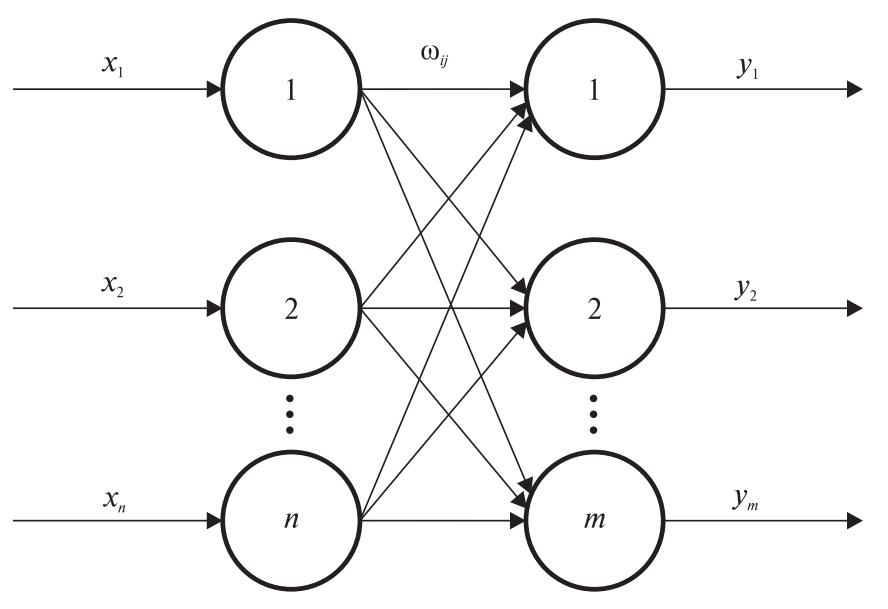
\includegraphics[width=0.4\linewidth]{figures/sd_ps/sd_ann/neural_network.png}}
	}

    \scnrelfrom{разбиение}{\scnkeyword{Типология и.н.с. по признаку направленности связей\scnsupergroupsign}}
    \scnaddlevel{1}
        \scneqtoset{
        искусственная нейронная сеть с прямыми связями\\
        \scnaddlevel{1}
            \scnsubdividing{
                персептрон\\
                \scnaddlevel{1}
                    \scnsubdividing{
                        персептрон Розенблатта;
                        автоэнкодерная искусственная нейронная сеть
                    }
                \scnaddlevel{-1}
                ;машина опорных векторов
                ;искусственная нейронная сеть радиально-базисных функций
            }
        \scnaddlevel{-1}
        ;искусственная нейронная сеть с обратными связями\\
        \scnaddlevel{1}
            \scnsubdividing{
                нейронная сеть Хопфилда
                ;нейронная сеть Хэмминга
            }
        \scnaddlevel{-1}
        ;рекуррентная искусственная нейронная сеть\\
        \scnaddlevel{1}
            \scnsubdividing{
            искусственная нейронная сеть Джордана
            ;искусственная нейронная сеть Элмана
            ;мультирекуррентная нейронная сеть
            ;LSTM-элемент
            ;GRU-элемент
            }
        \scnaddlevel{-1}
        }
    \scnaddlevel{-1}

    \scnrelfrom{разбиение}{\scnkeyword{Типология и.н.с. по признаку полноты связей\scnsupergroupsign}}
    \scnaddlevel{1}
        \scneqtoset{
        полносвязная искусственная нейронная сеть\\
        ;слабосвязная искусственная нейронная сеть
        }
    \scnaddlevel{-1}

    \scnrelfrom{решаемые задачи}{задачи, которые могут быть решены с помощью и.н.с. с приемлемой точностью}{
    \scnaddlevel{1}
    \scneqtoset{
        задача классификации\\
        \scnaddlevel{1}
            \scnsubset{задача}
            \scnexplanation{Задача построения классификатора, т.е. отображения $\tilde c: X \rightarrow C$, где $ X \in \mathbb{R}^m$ --
            признаковое пространство п.в.а., $C = {C_1, C_2, ...C_k }$ -- конечное и обычно небольшое множество меток классов.}
        \scnaddlevel{-1}
        ;задача регрессии\\
        \scnaddlevel{1}
            \scnsubset{задача}
            \scnexplanation{Задача построения оценочной функции по примерам $(x_i, f(x_i))$, где $f(x)$ -- неизвестная функция}
            \scnexplanation{\textbf{\textit{оценочная функция}} -- отображение вида $\tilde{f}: X \rightarrow \mathbb{R}$, где $X \in \mathbb{R}^m$ -- признаковое пространство п.в.а.}
        \scnaddlevel{-1}
        ;задача кластеризация\\
        \scnaddlevel{1}
            \scnsubset{задача}
            \scnexplanation{Задача разбиения множества п.в.а. на группы (кластеры) по какой-либо метрике сходства.}
        \scnaddlevel{-1}
        ;задача понижения размерности\\
        \scnaddlevel{1}
            \scnsubset{задача}
            \scnidtf{задача уменьшения размерности признакового пространства}
        \scnaddlevel{-1}
        ;задача управления\\
        \scnaddlevel{1}
            \scnsubset{задача}
        \scnaddlevel{-1}
        ;задача фильтрации\\
        \scnaddlevel{1}
            \scnsubset{задача}
        \scnaddlevel{-1}
        ;задача детекции\\
        \scnaddlevel{1}
            \scnsubset{задача}
            \scnsubset{задача классификации}
            \scnsubset{задача регрессии}
        \scnaddlevel{-1}
        ;задача с ассоциативной памятью\\
        \scnaddlevel{1}
            \scnsubset{задача}
        \scnaddlevel{-1}
    }
    }

\scnheader{формальный нейрон}
    \scnidtf{искусственный нейрон}
    \scnidtf{нейрон}
    \scnidtf{ф.н.}
    \scnidtf{нейронный элемент}
    \scnidtf{множество нейронов искусственных нейронных сетей}
    \scnidtf{математическая модель реального биологического нейрона}
    \scnnote{Отдельный формальный нейрон является искусственной нейронной сети с одним нейроном в единственном слое.}
    \scnsubset{искусственная нейронная сеть}
    \scnexplanation{\textbf{\textit{формальный нейрон}} -- это основной элемент \textit{искусственной нейронной сети}, применяющий свою \textit{функцию активации} (\scncite{Golovko2017}) к сумме произведений входных сигналов на весовые коэффициенты:
        \begin{equation*}
            y = F\left(\sum_{i=1}^{n} w_ix_i - T\right) = F(WX - T)
        \end{equation*}
        где $X = (x_1,x_2,...,x_n)^{T}$ -- вектор входного сигнала; $W - (w_1,w_2,...,w_n)$ -- вектор весовых коэффициентов; \textit{T} -- пороговое значение;
        \textit{F} -- функция активации.
    }

    \scnrelfrom{изображение}{
        \scnfileimage{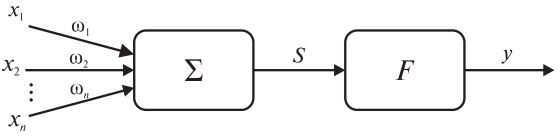
\includegraphics[width=0.4\linewidth]{figures/sd_ps/sd_ann/neuron.png}}
    }

    \scnnote{Формальные нейроны могут иметь полный набор связей с нейронами предшествующего слоя или неполный (разряженный)
        набор связей.}

    \scnsubdividing{
        полносвязный формальный нейрон\\
        \scnaddlevel{1}
            \scnidtf{нейрон, у которого есть полный набор связей с нейронами предшествующего слоя}
            \scnexplanation{отдельный обрабатывающий элемент и.н.с., выполняющий функциональное преобразование взвешенной суммы элементов вектора входных значений с помощью функции активации}
        \scnaddlevel{-1}
        ;сверточный формальный нейрон\\
        \scnaddlevel{1}
            \scnexplanation{Отдельный обрабатывающий элемент и.н.с., выполняющий функциональное преобразование результата
                операции свертки матрицы входных значений с помощью функции активации.}
            \scnnote{Сверточный формальный нейрон может быть представлен полносвязным формальным нейроном} 
            %\scnnote{Сверточный формальный нейрон с соответствующим ему ядром свертки может быть представлен нейроном с неполным набором связей.}
        \scnaddlevel{-1}
        ;рекуррентный формальный нейрон\\
        \scnaddlevel{1}
            \scnexplanation{Формальный нейрон, имеющий обратную связь с самим собой или с другими нейронами и.н.с.}
        \scnaddlevel{-1}
    }

\scnheader{формальный нейрон\scnrolesign}
    \scnidtf{формальный нейронный элемент\scnrolesign}
    \scnidtf{нейронный элемент\scnrolesign}
    \scnidtf{нейрон\scnrolesign}
    \scniselement{ролевое отношение}
    \scnrelfrom{первый домен}{искусственная нейронная сеть}
    \scnrelfrom{второй домен}{формальный нейрон}
    \scnrelfrom{область определения}{искусственная нейронная сеть}
    \scnexplanation{\textbf{\textit{формальный нейрон\scnrolesign}} -- ролевое отношение, связывающее искусственную нейронную сеть с ее нейроном.}

\scnheader{пороговый формальный нейрон\scnrolesign}
    \scnidtf{пороговый нейронный элемент\scnrolesign}
    \scnidtf{пороговый нейрон\scnrolesign}
    \scniselement{ролевое отношение}
    \scnrelfrom{первый домен}{искусственная нейронная сеть}
    \scnrelfrom{второй домен}{формальный нейрон}
    \scnrelfrom{область определения}{искусственная нейронная сеть}
    \scnexplanation{\textbf{\textit{пороговый формальный нейрон\scnrolesign}} -- ролевое отношение, связывающее искусственную нейронную сеть с таким ее нейроном,
            выходное значение которого всегда равно -1.
    }
    \scnexplanation{Весовой коэффициент синаптической связи, выходящей из такого нейрона, является порогом для нейрона, в который
        данная синаптическая связь входит.}

\scnheader{синаптическая связь}
    \scnidtf{синапс}
    \scnsubset{ориентированная пара}
    \scndefinition{\textbf{\textit{синаптическая связь}} -- ориентированная пара, первым компонентом которой является нейрон, из
        которого исходит сигнал, а вторым компонентом -- нейрон, который принимает этот сигнал.
    }

\scnheader{синаптическая связь\scnrolesign}
    \scnidtf{синапс\scnrolesign}
    \scniselement{ролевое отношение}
    \scnrelfrom{первый домен}{искусственная нейронная сеть}
    \scnrelfrom{второй домен}{синаптическая связь}
    \scnrelfrom{область определения}{\scnstartsetlocal\scnendstructlocal\\
        \scnreltoset{объединение}{искусственная нейронная сеть;синапс}
    }
    \scndefinition{\textbf{\textit{синаптическая связь\scnrolesign}} -- ролевое отношение, связывающее искусственную нейронную сеть с ее синапсом.
    }

\scnheader{параметр и.н.с.}
    \scnsubset{параметр}
    \scnsubdividing{
        настраиваемый параметр и.н.с.\\
        \scnaddlevel{1}
            \scnidtf{параметр и.н.с., значение которого изменяется в ходе обучения}
            \scnsubdividing{
                весовой коэффициент синаптической связи;
                пороговое значение;
                ядро свертки
                \scnaddlevel{1}
                    \scnidtf{квадратная матрица произвольного порядка, элементы которой изменяются в процессе
                        обучения и.н.с.}
                    \scnnote{если сверточный формальный нейрон представить в виде полносвязного формального нейрона, соответствующее ядро свертки преобразуется в вектор весовых коэффициентов}
                \scnaddlevel{-1}
            }
        \scnaddlevel{-1}\\
        ;архитектурный параметр и.н.с.\\
        \scnaddlevel{1}
            \scnnote{Параметр и.н.с., определяющий ее архитектуру.}
            \scnsubdividing{количество слоев;количество нейронов; количество синапсов}
        \scnaddlevel{-1}
    }

\scnheader{весовой коэффициент синаптической связи}
    \scnidtf{вес синапса}
    \scnidtf{сила синаптической связи}
    \scnsubset{настраиваемый параметр}
    \scnexplanation{\textbf{\textit{весовой коэффициент синаптической связи}} -- это числовой коэффициент, который ставится в соответствие каждому
        синапсу нейронной сети и изменяется в процессе обучения.
    }
    \scnnote{Если сила синаптической связи отрицательна, то она называется \textit{тормозящей}. В противном случае она
        является \textit{усиливающей}.
    }

\scnheader{входное значение формального нейрона*}
    \scnidtf{входное значение нейрона*}
    \scnidtf{входное значение*}
    \scniselement{неролевое отношение}
    \scniselement{бинарное отношение}
    \scnrelfrom{первый домен}{формальный нейрон}
    \scnrelfrom{второй домен}{число}
    \scnrelfrom{область определения}{\scnstartsetlocal\scnendstructlocal\\
        \scnreltoset{объединение}{формальный нейрон;число}
    }
    \scnexplanation{\textbf{\textit{входное значение формального нейрона*}} -- неролевое отношение, связывающее нейрон входного слоя со
        значением признака п.в.а., который подается на вход нейронной сети.
    }
    \scntext{теоретическая неточность}{Использование множества как формы представления входных данных является серьезным допущением, так как на практике
        входные данные структурированы более сложно -- в многомерные массивы. Самым близким теоретическим аналогом
        здесь выступает тензор. К сожалению, описание теории нейронных сетей с помощью тензорного исчисления в литературе
        как таковое отсутствует, но активно используется на практике: например, во многих разрабатываемых нейросетевых фреймворках.
        Формализация нейронных сетей с помощью тензоров видится авторам наиболее вероятным направлением работы в
        ближайших изданиях \textit{стандарта OSTIS}.
    }

\scnheader{паттерн входной активности и.н.с.}
	\scnidtf{п.в.а.}
    \scniselement{мультимножество}
    \scniselement{кортеж}
    \scnexplanation{\textbf{\textit{паттерн входной активности и.н.с.}} -- ориентированное мультимножество численных значений
        признаков некоторого объекта, которые могут выступать в качестве входных значений нейронов.
    }
	\scnnote{В текущей версии \textit{Стандарта OSTIS} предполагается, что п.в.а. содержит только предобработанные данные,
        то есть данные приведенные к численному виду и, возможно, преобразованные с помощью известных статистических
        методов (например, нормирования).
    }

\scnheader{признак}
    \scnidtf{feature}
    \scnidtf{множество признаков}
    \scnsubset{ролевое отношение}
    \scnexplanation{\textbf{\textit{признак}} -- множество ролевых отношений, каждое из которых связывает некоторый п.в.а. с численным значением, которое характеризует данный п.в.а. с какой-либо стороны.
    }

\scnheader{функция активации*}
    \scnidtf{функция активации нейрона*}
    \scniselement{неролевое отношение}
    \scniselement{бинарное отношение}
    \scnexplanation{\textbf{\textit{функция активации*}} -- неролевое отношение, связывающее формальный нейрон с функцией, результат
        применения которой к \textbf{\textit{взвешенной сумме нейрона}} определяет его \textbf{\textit{выходное значение}}.
    }
    \scnrelfrom{область определения}{\scnstartsetlocal\scnendstructlocal\\
        \scnreltoset{объединение}{формальный нейрон;функция}
    }
    \scnrelfrom{первый домен}{формальный нейрон}
    \scnrelfrom{второй домен}{функция}
    \scnaddlevel{1}
    \scnsubdividing{
        линейная функция\\
        \scnaddlevel{1}
            \scntext{формула}{
                \begin{equation*}
                    y = kS
                \end{equation*}
                где \textit{k} -- коэффициент наклона прямой, \textit{S} -- в.с.
            }
        \scnaddlevel{-1}
        ;пороговая функция\\
        \scnaddlevel{1}
            \scntext{формула}{
                \begin{equation*}
                    y = sign(S) =
                    \begin{cases}
                        1, S > 0,\\
                        0, S \leq 0
                    \end{cases}
                \end{equation*}
            }
        \scnaddlevel{-1}
        ;сигмоидная функция\\
        \scnaddlevel{1}
            \scntext{формула}{
                \begin{equation*}
                    y = \frac{1}{1+e^{-cS}}
                \end{equation*}
                где \textit{с} > 0 -- коэффициент, характеризующий ширину сигмоидной функции по оси абсцисс, \textit{S} -- в.с.
            }
        \scnaddlevel{-1}
        ;функция гиперболического тангенса\\
        \scnaddlevel{1}
            \scntext{формула}{
                \begin{equation*}
                    y = \frac{e^{cS}-e^{-cS}}{e^{cs}+e^{-cS}}
                \end{equation*}
                где \textit{с} > 0 -- коэффициент, характеризующий ширину сигмоидной функции по оси абсцисс, \textit{S} -- в.с.
            }
        \scnaddlevel{-1}
        ;функция softmax\\
        \scnaddlevel{1}
            \scntext{формула}{
                \begin{equation*}
                    y_j = softmax(S_j) = \frac{e^{S_j}}{\sum_{j} e^{S_j}}
                \end{equation*}
                где $S_j$ -- в.с. \textit{j}-го выходного нейрона
            }
        \scnaddlevel{-1}
        ;функция ReLU\\
        \scnaddlevel{1}
            \scntext{формула}{
                \begin{equation*}
                    y = F(S) =
                    \begin{cases}
                        S, S > 0,\\
                        kS, S \leq 0
                    \end{cases}
                \end{equation*}
                где \textit{k} = 0 или принимает небольшое значение, например, 0.01 или 0.001.
            }
        \scnaddlevel{-1}
    }
    \scnaddlevel{-1}

\scnheader{взвешенная сумма*}
    \scnidtf{взвешенная сумма входных значений*}
    \scnidtf{в.с.}
    \scniselement{неролевое отношение}
    \scniselement{бинарное отношение}
    \scnexplanation{\textbf{\textit{взвешенная сумма*}} -- неролевое отношение, связывающее формальный нейрон с числом, являющимся суммой
        произведений входных сигналов на весовые коэффициенты входящих в нейрон синаптических связей.
    }
    \scnrelfrom{область определения}{\scnstartsetlocal\scnendstructlocal\\
        \scnreltoset{объединение}{формальный нейрон;число}
    }
    \scnrelfrom{первый домен}{формальный нейрон}
    \scnrelfrom{второй домен}{число}
    \scnrelfrom{формула}{
        \begin{equation*}
            S = \sum_{i=1}^{n} w_ix_i - T
        \end{equation*}
        где \textit{n} -- размерность вектора входных значений, $w_i$ -- \textit{i}-тый элемент вектора весовых
        коэффициентов, $x_i$ -- \textit{i}-тый элемент вектора входных значений, \textit{T} -- пороговое значение.
    }

\scnheader{выходное значение формального нейрона*}
    \scnidtf{выходное значение нейрона*}
    \scnidtf{выходное значение*}
    \scniselement{неролевое отношение}
    \scniselement{бинарное отношение}
    \scnrelfrom{первый домен}{формальный нейрон}
    \scnrelfrom{второй домен}{число}
    \scnrelfrom{область определения}{\scnstartsetlocal\scnendstructlocal\\
        \scnreltoset{объединение}{формальный нейрон;число}
    }
    \scnexplanation{\textbf{\textit{входное значение*}} -- неролевое отношение, связывающее нейрон с числом, являющимся результатом применения
        функции активации нейрона к его взвешенной сумме.
    }
    \scnnote{Выходное значение нейрона является одним из входных сигналов для всех нейронов, в которые ведут выходящие из данного нейрона синапсы.
    }

\scnheader{слой и.н.с.}
    \scnidtf{слой}
    \scnidtf{слой искусственной нейронной сети}
    \scnidtf{множество слоев искусственных нейронных сетей}
    \scnnote{отдельный слой является искусственной нейронной сетью с одним слоем}
    \scnsubset{искусственная нейронная сеть}
    \scnexplanation{\textbf{\textit{слой и.н.с}}  -- это множество нейронных элементов, на которые в каждый такт времени
        параллельно поступает информация от других нейронных элементов сети (\scncite{Golovko2017})
    }
    \scnexplanation{\textbf{\textit{слой и.н.с.}} -- это множество формальных нейронов, осуществляющих параллельную независимую обработку
        вектора или матрицы входных значений
    }
    \scnnote{функция активации слоя является функцией активации всех формальных нейронов этого слоя}
    \scnnote{конфигурация слоя задается типом, количеством формальных нейронов, функцией активации}
    \scnnote{описание последовательности слоев и.н.с. с конфигурацией каждого слоя задает архитектуру и.н.с.}

    \scnsubdividing{
        полносвязный слой и.н.с.\\
        \scnaddlevel{1}
            \scnidtf{слой, в котором каждый нейрон имеет связь с каждым нейроном предшествующего слоя}
            \scnidtf{слой, в котором каждый нейрон является полносвязным}
        \scnaddlevel{-1}
        ;сверточный слой и.н.с.\\
        \scnaddlevel{1}
            \scnidtf{слой, в котором каждый нейрон является сверточным}
        \scnaddlevel{-1}
        ;слой и.н.с. нелинейного преобразования\\
        \scnaddlevel{1}
            \scnidtf{слой, осуществляющий нелинейное преобразование входных данных}
            \scnexplanation{Как правило, выделяются в отдельные слои только в программных реализациях. Фактически
                рассматриваются как финальный этап расчета выходной активности любого нейрона -- применение функции
                активации.}
            \scnnote{не изменяет размерность входных данных}
        \scnaddlevel{-1}
        ;dropout слой и.н.с.\\
        \scnaddlevel{1}
            \scnidtf{слой, реализующий технику регуляризации dropout}
            \scnnote{Данный тип слоя функционирует только во время обучения и.н.с.}
            \scnexplanation{Поскольку полносвязные слои имеют большое количество настраиваемых параметров, они
                подвержены эффекту переобучения. Один из способов устранить такой негативный эффект -- выполнить
                частичный отсев результатов на выходе полносвязного слоя. На этапе обучения техника dropout позволяет
                отбросить выходную активность некоторых нейронов с определенной, заданной вероятностью. Выходная
                активность ``отброшенных'' нейронов полагается равной нулю.}
        \scnaddlevel{-1}
        ;pooling слой и.н.с.\\
        \scnaddlevel{1}
            \scnidtf{подвыборочный слой}
            \scnidtf{объединяющий слой}
            \scnidtf{слой, осуществляющий уменьшение размерности входных данных}
        \scnaddlevel{-1}
        ;слой и.н.с. батч-нормализации\\
    }

\scnheader{распределяющий слой*}
    \scnidtf{входной слой*}
    \scniselement{неролевое отношение}
    \scniselement{бинарное отношение}
    \scndefinition{\textbf{\textit{распределяющий слой*}} -- неролевое отношение, связывающее искусственную нейронную сеть с ее слоем,
        нейроны которого принимают входные значения всей нейронной сети.
    }
    \scnrelfrom{область определения}{искусственная нейронная сеть}
    \scnrelfrom{первый домен}{искусственная нейронная сеть}
    \scnrelfrom{второй домен}{слой и.н.с.}

\scnheader{обрабатывающий слой*}
    \scniselement{неролевое отношение}
    \scniselement{бинарное отношение}
    \scndefinition{\textbf{\textit{обрабатывающий слой*}} -- неролевое отношение, связывающее искусственную нейронную сеть с ее слоем,
        нейроны которого принимают на вход выходные значения нейронов предыдущего слоя.
    }
    \scnrelfrom{область определения}{искусственная нейронная сеть}
    \scnrelfrom{первый домен}{искусственная нейронная сеть}
    \scnrelfrom{второй домен}{слой и.н.с}

\scnheader{выходной слой*}
    \scniselement{неролевое отношение}
    \scniselement{бинарное отношение}
    \scnexplanation{\textbf{\textit{выходной слой*}} -- неролевое отношение, связывающее искусственную нейронную сеть с ее слоем,
        выходные значения нейронов которого являются выходными значениями всей нейронной сети.
    }
    \scnrelfrom{область определения}{искусственная нейронная сеть}
    \scnrelfrom{первый домен}{искусственная нейронная сеть}
    \scnrelfrom{второй домен}{слой и.н.с}

\bigskip
\scnendstruct \scnendsegmentcomment{Предметная область и онтология искусственных нейронных сетей}

\scnsegmentheader{Предметная область и онтология действий по обработке искусственной нейронной сети}
\scnstartsubstruct

\newpage
\scnheader{Предметная область действий по обработке искусственных нейронных сетей}
    \scnidtf{Предметная область действий по обработке и.н.с.}
    \scniselement{предметная область}
    \scnsdmainclass{действие по обработке искусственных нейронных сетей}
    \scnsdclass{
        действие по обработке искусственных нейронных сетей;
        действие конфигурации весовых коэффициентов и.н.с.;
        действие конфигурации и.н.с.;
        действие интерпретации и.н.с.;
        метод обучения и.н.с.;
        метод обучения с учителем;
        метод обратного распространения ошибки;
        метод обучения без учителя;
        метод оптимизации;
        функция потерь;
        параметр обучения;
        скорость обучения;
        моментный параметр;
        параметр регуляризации;
        размер группы обучения;
        количество эпох обучения;
        выборка
    }
    \scnsdrelation{
        обучающая выборка\scnrolesign;
        тестовая выборка\scnrolesign;
        валидационная выборка\scnrolesign;
        метод обучения\scnrolesign;
        метод оптимизации\scnrolesign;
        функция потерь\scnrolesign
    }

\scnheader{действие по обработке искусственной нейронной сети}
    \scnidtf{действие по обработке и.н.с.}
    \scnidtf{действие с искусственной нейронной сетью}
    \scnsubset{действие}
    \scnexplanation{В зависимости от того, является ли искусственная нейронная сеть знаком внешней по отношению к памяти системы сущности,
        элементы множества действие по обработке и.н.с. являются либо элементами множества \textbf{\textit{действие, выполняемое кибернетической
        системой в своей внешней среде}}, либо элементом множества \textbf{\textit{действие, выполняемое кибернетической системой
        в собственной памяти.
    }}.
    }
    \scnsubdividing{
        действие конфигурации и.н.с.\\
        \scnaddlevel{1}
        \scnsubdividing{
            действие создания и.н.с.
            ;действие редактирования и.н.с.
            ;действие удаления и.н.с.
            ;действие конфигурации слоя и.н.с.\\
            \scnaddlevel{1}
                \scnsubdividing{
                    действие добавления слоя в и.н.с.
                    ;действие редактирования слоя и.н.с.
                    ;действие удаления слоя и.н.с.
                    ;действие установки функции активации нейронов слоя и.н.с.
                    ;действие конфигурации нейрона в слое и.н.с\\
                    \scnaddlevel{1}
                        \scnsubdividing{
                            действие добавления нейрона в слой и.н.с.
                            ;действие редактирования нейрона в слое и.н.с.
                            ;действие удаления нейрона из слоя и.н.с.
                            ;действие установки функции активации нейрона в слое и.н.с.
                        }
                    \scnaddlevel{-1}
                }
            \scnaddlevel{-1}
        }
        \scnaddlevel{-1}
        ;действие конфигурации весовых коэффициентов и.н.с.\\
        \scnaddlevel{1}
            \scnsuperset{действие обучения и.н.с.}
            \scnsuperset{действие начальной инициализации весов и.н.с.}
            \scnaddlevel{1}
                \scnsuperset{действие начальной инициализации весов нейронов слоя и.н.с.}
                \scnaddlevel{1}
                    \scnsuperset{действие начальной инициализации весов нейрона и.н.с.}
                \scnaddlevel{-1}
            \scnaddlevel{-1}
        \scnaddlevel{-1}
        ;действие интерпретации и.н.с.
    }
    \scnnote{Действия по обработке и.н.с осуществляет соответствующий коллектив агентов.}
    \scnexplanation{Так как в результате действий по обработке и.н.с объект этих действий, конкретная и.н.с, может существенно меняться
        (меняется конфигурация сети, ее весовые коэффициенты), то и.н.с представляется в базе знаний как темпоральное объединение
        всех ее версий. Каждая версия является и.н.с. и темпоральной сущностью. На множестве этих темпоральных сущностей задается
        темпоральная последовательность с указанием первой и последней версии. Для каждой версии описываются специфичные знания.
        Общие для всех версий знания описываются для и.н.с, являющейся темпоральным объединением всех версий.
    }
    \scnaddlevel{1}
        \scnrelfrom{пример}{
            \scnfilescg{figures/sd_ps/sd_ann/temporal_neural_network_scg.png}
        }
    \scnaddlevel{-1}

\scnheader{действие обучения и.н.с.}
    \scnidtf{действие обучения искусственной нейронной сети}
    \scnsubset{действие конфигурации весовых коэффициентов и.н.с.}
    \scndefinition{\textbf{\textit{действие обучения и.н.с.}} -- действие, в ходе которого реализуется определенный метод обучения
        и.н.с. с заданными параметрами обучения и.н.с, методом оптимизации и функцией потерь.
    }
    \scnrelfromset{известные проблемы}{
        \scnfileitem{Переобучение -- проблема, возникающая при обучении и.н.с., заключающаяся в том,
        что сеть хорошо адаптируется к п.в.а. из обучающей выборки, при этом теряя способность к обобщению.
        Переобучение возникает из-за применения неоправданно сложной модели при обучении и.н.с. Это происходит,
        когда количество настраиваемых параметров и.н.с. намного больше размера обучающей выборки. Возможные
        варианты решения проблемы заключаются в упрощении модели, увеличении выборки, использовании регуляризации
        (параметр регуляризации, техника dropout и т.д.).\\
        Обнаружение переобученности сложнее, чем недообученности. Как правило, для этого применяется
        кросс-валидация на валидационной выборке, позволяющая оценить момент завершения процесса обучения.
        Идеальным вариантом является достижение баланса между переобученностью и недообученностью.
        };
        \scnfileitem{Недообучение -- проблема, возникающая при обучении и.н.с., заключающаяся в том,
        что сеть дает одинаково плохие результаты на обучающей и контрольной выборках.
        Чаще всего такого рода проблема возникает при недостаточном времени, затраченном на обучение модели.
        Однако это может быть вызвано и слишком простой архитектурой модели либо малым размером обучающей
        выборки. Соответственно решение, которое может быть принято ML-инженером, заключается в устранении
        этих недостатков: увеличение времени обучения, использование модели с большим числом настраиваемых
        параметров, увеличение размера обучающей выборки, а также уменьшение регуляризации и более тщательный
        отбор признаков для обучающих примеров.
        }
    }
    \scnrelfrom{описание примера}{
        \scnfilescg{figures/sd_ps/sd_ann/ann_trainning_scg.png}
    }

\scnheader{выборка}
    \scnsubset{множество}
	\scnexplanation{\textbf{\textit{выборка}} -- множество п.в.а., используемых в процессе обучения, тестирования
        и архитектурной настройки и.н.с.
    }

\scnheader{обучающая выборка\scnrolesign}
    \scnidtf{training set\scnrolesign}
    \scniselement{ролевое отношение}
    \scnrelfrom{первый домен}{действие обучения и.н.с.}
    \scnrelfrom{второй домен}{выборка}
    \scnrelfrom{область определения}{\scnstartsetlocal\scnendstructlocal\\
        \scnreltoset{объединение}{действие обучения и.н.с.;выборка}
    }
    \scnexplanation{\textbf{\textit{обучающая выборка\scnrolesign}} -- ролевое отношение, связывающее действие обучения и.н.с. с выборкой,
        используемой для изменения настраиваемых параметров и.н.с. в процессе ее обучения.
    }

\scnheader{тестовая выборка\scnrolesign}
    \scnidtf{test set\scnrolesign}
    \scniselement{ролевое отношение}
    \scnrelfrom{первый домен}{действие обучения и.н.с.}
    \scnrelfrom{второй домен}{выборка}
    \scnrelfrom{область определения}{\scnstartsetlocal\scnendstructlocal\\
        \scnreltoset{объединение}{действие обучения и.н.с.;выборка}
    }
    \scnexplanation{\textbf{\textit{тестовая выборка\scnrolesign}} -- ролевое отношение, связывающее действие обучения и.н.с. с выборкой,
        используемой для проверки обобщающей способности обученной и.н.с.
    }
    \scnnote{Элементы контрольной выборки не используются в процессе обучения.}
\right) 
\scnheader{валидационная выборка\scnrolesign}
    \scniselement{ролевое отношение}
    \scnrelfrom{первый домен}{действие обучения и.н.с.}
    \scnrelfrom{второй домен}{выборка}
    \scnrelfrom{область определения}{\scnstartsetlocal\scnendstructlocal\\
        \scnreltoset{объединение}{действие обучения и.н.с.;выборка}
    }
    \scnexplanation{\textbf{\textit{валидационная выборка\scnrolesign}} -- ролевое отношение, связывающее действие обучения и.н.с. с выборкой,
        используемой для определения (настройки) архитектурных параметров и.н.с. и параметров обучения.
    }
    \scnnote{Элементы валидационной выборки не используются в процессе обучения (не входят в обучающую выборку).}


\scnheader{метод обучения и.н.с.}
    \scnsubset{метод}
	\scnexplanation{\textbf{\textit{метод обучения и.н.с.}} -- метод итеративного поиска оптимальных значений настраиваемых параметров и.н.с.,
        минимизирующих некоторую заданную функцию потерь.
    }
	\scnnote{Стоит отметить, что хотя целью применения метода обучения является минимизация функции потерь, ``полезность''
        полученной после обучения модели можно оценить только по достигнутому уровню ее обобщающей способности.
    }
	\scnsuperset{метод обучения с учителем}
	\scnaddlevel{1}
		\scnexplanation{
            \textbf{\textit{метод обучения с учителем}} -- метод обучения с использованием заданных целевых переменных.
        }
		\scnsuperset{метод обратного распространения ошибки}
		\scnaddlevel{1}
			\scnidtf{м.о.р.о.}
			\scntext{алгоритм}{\\
				\begin{minipage}{\linewidth}
					\vspace{-\baselineskip}
					\begin{algorithm}[H]
						\KwData{$X$ -- данные, $Et$ -- желаемый отклик (метки), $E_m$ -- желаемая ошибка (в соответствии с выбранной функцией потерь)}
						\KwResult{обученная нейронная сеть \textit{Net}}
						инициализация весов \textit{W} и порогов \textit{T};\\
						\Repeat{$E<E_m$}{
							\ForEach{$x \in X$ \And $e \in Et$}{
								фаза прямого распространения сигнала: вычисляются активации для всех слоев и.н.с.;\\
								фаза обратного распространения ошибки: вычисляются ошибки для последнего слоя и всех предшествующих слоев;\\
								изменение настраиваемых параметров и.н.с. в соответствии с вычисленными ошибками;\\
							}
							вычисление общей ошибки E на данной эпохе;
						}
					\end{algorithm}
				\end{minipage}
            }
			\scnnote{м.о.р.о. использует заданный метод оптимизации и заданную функцию потерь для реализации фазы
                обратного распространения ошибки и изменения настраиваемых параметров и.н.с. Одним из самых распространенных
                методов оптимизации является метод стохастического градиентного спуска. Приведенный м.о.р.о. используется
                для реализации последовательного варианта обучения.
            }
			\scnnote{Следует также отметить, что несмотря на то, что метод отнесен к методам обучения с учителем, в случае
                использования м.о.р.о. для обучения автокодировщиков в классических публикациях он рассматривается как
                метод обучения без учителя, поскольку в данном случае размеченные данные отсутствуют.
            }
		\scnaddlevel{-1}
	\scnaddlevel{-1}
	\scnsuperset{метод обучения без учителя}
	\scnaddlevel{1}
		\scnexplanation{\textbf{\textit{метод обучения без учителя}} -- метод обучения без использования заданных целевых переменных
            (в режиме самоорганизации)
        }
		\scnexplanation{В ходе выполнения алгоритма метода обучения без учителя выявляются полезные структурные свойства
            набора. Неформально его понимают как метод для извлечения информации из распределения, выборка для которого
            не была вручную аннотирована человеком (\scncite{Goodfellow2017}).
        }
	\scnaddlevel{-1}

\scnheader{метод обучения\scnrolesign}
    \scniselement{ролевое отношение}
    \scnrelfrom{первый домен}{действие обучения и.н.с.}
    \scnrelfrom{второй домен}{метод обучения и.н.с.}
    \scnrelfrom{область определения}{\scnstartsetlocal\scnendstructlocal\\
        \scnreltoset{объединение}{действие обучения и.н.с.;метод обучения и.н.с.}
    }
    \scnexplanation{\textbf{\textit{метод обучения\scnrolesign}} -- ролевое отношение, связывающее действие обучения и.н.с. с методом обучения,
        использующимся для обучения и.н.с. в рамках этого действия.
    }

\newpage
\scnheader{метод оптимизации}
    \scnsubset{метод}
	\scndefinition{\textbf{\textit{метод оптимизации}} -- метод для минимизации целевой функции потерь при обучении и.н.с.}
	\scnrelfromlist{включение}{
		SGD\\
		\scnaddlevel{1}
			\scnidtf{стохастический градиентный спуск}
			\scnidtf{с.г.с.}
			\scnidtf{stochastic gradient descent}
			\scnnote{В методе стохастического градиентного спуска корректировка настраиваемых параметров и.н.с. выполняется в направлении максимального уменьшения функции стоимости, т.е. в направлении, противоположном вектору градиента функции потерь (\scncite{Haykin2006})}
		\scnaddlevel{-1}
		;Nesterov method\\
		\scnaddlevel{1}
			\scnidtf{метод Нестерова}
			\scnnote{Обучение методом с.г.с. иногда происходит очень медленно. Импульсный метод позволяет ускорить обучение, особенно в условиях высокой кривизны, небольших, но устойчивых градиентов или зашумленных градиентов. В импульсном методе вычисляется экспоненциально затухающее скользящее среднее прошлых градиентов и продолжается движение в этом направлении. Метод Нестерова является вариантом импульсного алгоритма, в котором градиент вычисляется после применения текущей скорости (\scncite{Goodfellow2017})}
		\scnaddlevel{-1}
		;AdaGrad\\
		\scnaddlevel{1}
			\scnidtf{adaptive gradient}
			\scnnote{Данный метод по отдельности адаптирует скорости обучения всех настраиваемых параметров и.н.с., умножая их на коэффициент, обратно пропорциональный квадратному корню из суммы всех прошлых значений квадрата градиента (\scncite{Duchi2011})}
		\scnaddlevel{-1}
		;RMSProp\\
		\scnaddlevel{1}
			\scnidtf{root mean square propagation}
			\scnnote{Данный метод является модификацией AdaGrad, которая позволяет улучшить его поведение в невыпуклом случае путем изменения способа агрегирования градиента на экспоненциально взвешенное скользящее среднее. Использование экспоненциально взвешенного скользящего среднего гарантирует повышение скорости сходимости после обнаружения выпуклой впадины, как если бы внутри этой впадины алгоритм AdaGrad был инициализирован заново (\scncite{Goodfellow2017})}
		\scnaddlevel{-1}	
		;Adam\\
		\scnaddlevel{1}
			\scnidtf{adaptive moments}
			\scnnote{Данный метод можно рассматривать как комбинацию RMSProp и AdaGrad (\scncite{Kingma2014}). Помимо усредненного первого момента, данный метод использует усредненное значение вторых моментов градиентов}
		\scnaddlevel{-1}
	}
	\scnnote{Успешность применения методов оптимизации зависит главным образом от знакомства пользователя с соответствующим
        алгоритмом (\scncite{Goodfellow2017}).
    }

\scnheader{метод оптимизации\scnrolesign}
    \scniselement{ролевое отношение}
    \scnrelfrom{первый домен}{метод обучения и.н.с.}
    \scnrelfrom{второй домен}{метод оптимизации}
    \scnrelfrom{область определения}{\scnstartsetlocal\scnendstructlocal\\
        \scnreltoset{объединение}{метод обучения и.н.с.;метод оптимизации}
    }
    \scnexplanation{\textbf{\textit{метод оптимизации\scnrolesign}} -- ролевое отношение, связывающее метод обучения и.н.с. с методом оптимизации,
        использующимся для обучения и.н.с. с помощью данного метода.
    }

\scnheader{функция потерь}
    \scnsubset{функция}
	\scnexplanation{\textbf{\textit{функция потерь}} -- функция, используемая для вычисления ошибки, рассчитываемой как разница между фактическим
        эталонным значением и прогнозируемым значением, получаемым и.н.с.
    }
    \scnrelfromlist{включение}{
		MSE\\
		\scnaddlevel{1}
			\scnidtf{mean square error}
			\scnidtf{средняя квадратичная ошибка}
			\scntext{формула}{
				\begin{equation*}
					MSE = \frac{1}{L} \sum_{l=1}^L \sum_{i=1}^m (y_i^l - e_i^l)^2
				\end{equation*}
				где $y_i^l$ -- прогноз модели, $e_i^l$ -- ожидаемый (эталонный) результат, \textit{m} -- размерность выходного вектора, \textit{L} -- объем обучающей выборки.
			}
		\scnaddlevel{-1}
		;BCE\\
		\scnaddlevel{1}
			\scnidtf{binary cross entropy}
			\scnidtf{бинарная кросс-энтропия}
			\scntext{формула}{
				\begin{equation*}
					BCE = - \sum_{l=1}^L (e^l \log(y^l) + (1 - e^l)\log(1 - y^l))
				\end{equation*}
				где $y^l$ -- прогноз модели, $e^l$ -- ожидаемый (эталонный) результат: \textit{0} или \textit{1}, \textit{L} -- объем обучающей выборки.
			}
			\scnnote{для бинарной кросс-энтропии в выходном слое и.н.с. будет находиться один нейрон}
		\scnaddlevel{-1}
		;MCE\\
		\scnaddlevel{1}
			\scnidtf{multi-class cross entropy}
			\scnidtf{мультиклассовая кросс-энтропия}
			\scntext{формула}{
				\begin{equation*}
					MCE = - \sum_{l=1}^L \sum_{i=1}^m e_{i}^l \log(y_{i}^l)
				\end{equation*}
				где $y_{i}^l$ -- прогноз модели, $e_i^l$ -- ожидаемый (эталонный результат), \textit{m} -- размерность выходного вектора
			}
			\scnnote{для мультиклассовой кросс-энтропии количество нейронов в выходном слое и.н.с. совпадает с количеством классов}
		\scnaddlevel{-1}
	}
	\scnnote{Для решения задачи классификации рекомендуется использовать бинарную или мультиклассовую кросс-энтропийную функцию потерь,
        для решения задачи регрессии рекомендуется использовать среднюю квадратичную ошибку.
    }

\scnheader{функция потерь\scnrolesign}
    \scniselement{ролевое отношение}
    \scnrelfrom{первый домен}{метод обучения и.н.с.}
    \scnrelfrom{второй домен}{функция потерь}
    \scnrelfrom{область определения}{\scnstartsetlocal\scnendstructlocal\\
        \scnreltoset{объединение}{метод обучения и.н.с.;функция потерь}
    }
    \scnexplanation{\textbf{\textit{функция потерь\scnrolesign}} -- ролевое отношение, связывающее метод обучения и.н.с. с функцией потерь,
        использующимся для обучения и.н.с. с помощью данного метода.
    }

\scnheader{параметр обучения}
   \scnidtf{группа наиболее общих параметров метода обучения и.н.с.}
   \scnrelfromset{состав группы параметров обучения}{
       скорость обучения\\
          \scnaddlevel{1}
              \scnexplanation{\textbf{\textit{скорость обучения}} -- параметр, определяющий скорость изменения параметров и.н.с.
                в процессе обучения.
              }
          \scnaddlevel{-1}
       ;моментный параметр\\
          \scnaddlevel{1}
                \scnidtf{момент}
                \scnidtf{momentum}
                \scnexplanation{\textbf{\textit{моментный параметр}} -- параметр, используемый в процессе обучения для устранения
                    проблемы ``застревания'' алгоритма обучения в локальных минимумах минимизируемой функции потерь.
                }
                \scnexplanation{При обучении и.н.с. частой является ситуация остановки процесса в определенной точке локального
                    минимума без достижения желаемого уровня обобщающей способности и.н.с. Для устранения такого
                    нежелательного явления вводится дополнительный параметр (момент) позволяющий алгоритму обучения
                    ``перескочить'' через локальный минимум и продолжить процесс.
                }
         \scnaddlevel{-1}
       ;параметр регуляризации\\
         \scnaddlevel{1}
             \scnexplanation{\textbf{\textit{параметр регуляризации}} -- параметр, применяемый для контроля уровня переобучения и.н.с.
             }
             \scnexplanation{\textbf{\textit{регуляризация}} -- добавление дополнительных ограничений к правилам изменения настраиваемых
                параметров и.н.с. с целью предотвратить переобучение.
             }
         \scnaddlevel{-1}
       ;размер группы обучения\\
         \scnaddlevel{1}
             \scnexplanation{\textbf{\textit{размер группы обучения}} -- размер группы п.в.а., которая используется для изменения параметров
                и.н.с. на каждом элементарном шаге обучения.
             }
         \scnaddlevel{-1}
       ;количество эпох обучения\\
       \scnaddlevel{1}
       		\scnexplanation{\textbf{\textit{эпоха обучения}} -- одна итерация алгоритма обучения, в ходе которой все обучающие п.в.а.
                из обучающей выборки были однократно использованы.
            }
       \scnaddlevel{-1}
   }

\bigskip
\scnendstruct \scnendsegmentcomment{Предметная область и онтология действий по обработке искусственной нейронной сети}

\bigskip
\scnendstruct \scnendcurrentsectioncomment

\end{SCn}

\scsubsubsection[\scnrelfrom{ответственный автор}{Ковалев М.В.}\protect\scneditors{Крощенко А.А.;Головко В.А.}\protect\scnmonographychapter{Глава 3.6. Конвергенция и интеграция искусственных нейронных сетей с базами знаний в интеллектуальных компьютерных системах нового поколения}]{Предметная область и онтология синтаксиса sc-моделей искусственных нейронных сетей}
\label{sd_syntax_sc_model_ann}

\scsubsubsection[\scnrelfrom{ответственный автор}{Ковалев М.В.}\protect\scneditors{Крощенко А.А.;Головко В.А.}\protect\scnmonographychapter{Глава 3.6. Конвергенция и интеграция искусственных нейронных сетей с базами знаний в интеллектуальных компьютерных системах нового поколения}]{Предметная область и онтология денотационной семантики sc-моделей искусственных нейронных сетей}
\label{sd_denot_sem_sc_model_ann}

\scsubsubsection[\scnrelfrom{ответственный автор}{Ковалев М.В.}\protect\scneditors{Крощенко А.А.;Головко В.А.}\protect\scnmonographychapter{Глава 3.6. Конвергенция и интеграция искусственных нейронных сетей с базами знаний в интеллектуальных компьютерных системах нового поколения}]{Предметная область и онтология операционной семантики sc-моделей искусственных нейронных сетей}
\label{sd_oper_sem_sc_model_ann}